\documentclass{report}
\usepackage{fullpage}
\usepackage{imakeidx}\makeindex
\usepackage{hyperref}
\usepackage[nottoc,notlot,notlof]{tocbibind}
\usepackage[toc]{glossaries}\makeglossaries
\usepackage{graphicx}
\usepackage{framed}
\usepackage{tcolorbox}
\usepackage{verbatim}
\usepackage{fancyvrb}
\usepackage{comment}
\usepackage{amsmath}
\usepackage{geometry}
\usepackage{enumitem}
\usepackage{etoolbox}

\AtBeginEnvironment{enumerate}{\everymath{\displaystyle}}
\newlist{problems}{enumerate}{2}
\setlist[problems]{wide=0pt}
\setlist[problems,1]{label=\thechapter.\arabic*, font=\bfseries, wide=0pt}
\setlist[problems,2]{label=(\alph*), wide =0.5em, topsep=2pt, itemsep=2pt}

\widowpenalty 10000
\clubpenalty 10000
\tolerance=9999
\newcommand{\tm}{\raisebox{.9ex}{\tiny tm}}

\newglossaryentry{actor model}
{
  name=actor model,
  description={is a concurrency model where there are no shared variables, only
      processes with private variables that communicate through message passing}
}
\newglossaryentry{atomicity}
{
  name=atomicity,
  description={describes that a certain machine instruction or sequence of machine
    instructions by a process is executed indivisibly and cannot be interleaved with 
    machine instructions of another process}
}
\newglossaryentry{barrier synchronization}
{
  name=barrier synchronization,
  description={is when a set of processes execute in rounds, waiting for one another
    to complete each round}
}
\newglossaryentry{blocked process}
{
  name=blocked process,
  description={is a process that is waiting on a low-level synchronization primitive
    and cannot make progress without the help of another process.
      For example, a process that is waiting for a spinlock to become available}
}
\newglossaryentry{busy waiting}
{
  name=busy waiting,
  description={(aka spin-waiting) is when a process waits in a loop for some
      application-defined condition}
}
\newglossaryentry{concurrent execution}
{
  name=concurrent execution,
  description={(aka parallel execution) is when there are multiple processes executing and
      their machine instructions are interleaved in an unpredictable manner}
}
\newglossaryentry{condition variable}
{
  name=condition variable,
  description={a variable that keeps track of which processes are waiting for a
    specific application-level condition.  The variable can be waited on as well
    as signaled or notified}
}
\newglossaryentry{context}
{
  name=context,
  description={(aka continuation) describes the state of a running process,
    including its program counter, the values of its variables (stored in its
    register), and the contents of its stack}
}
\newglossaryentry{conditional critical section}
{
  name=conditional critical section,
  description={is a critical section with, besides mutual exclusion, additional conditions on
      when a process is allowed to enter the critical section}
}
\newglossaryentry{critical section}
{
  name=critical section,
  description={(aka critical region) is a set of instructions that only one process
    is allowed to execute at a time.  The instructions are, however, not executed
    atomically, as other processes can continue to execute and access shared
    variables}
}
\newglossaryentry{deadlock}
{
  name=deadlock,
  description={is when there are two or more processes waiting indefinitely for one
    another to release a resource}
}
\newglossaryentry{determinism}
{
  name=determinism,
  description={is when the outcome of an execution is uniquely determined by the
    initial state}
}
\newglossaryentry{fairness}
{
  name=fairness,
  description={is when each process eventually can access each resource it needs to access
    with high probability}
}
\newglossaryentry{interlock instruction}
{
  name=interlock instruction,
  description={a machine instruction that involves multiple memory load and/or store
    operations, executed atomically}
}
\newglossaryentry{invariant}
{
  name=invariant,
  description={is a binary predicate over states that must hold for every
  reachable state of a process}
}
\newglossaryentry{lock}
{
  name=lock,
  description={an object that can be owned by at most one process at a time.  Useful
    for implementing mutual exclusion}
}
\newglossaryentry{machine instruction}
{
  name=machine instruction,
  description={is an atomic operation on the CXL virtual machine, executed by a process}
}
\newglossaryentry{model checking}
{
  name=model checking,
  description={is a formal verification method that explores all possible executions
    of a program, which must have a finite number of states}
}
\newglossaryentry{monitor}
{
  name=monitor,
  description={is a programming language paradigm that supports mutual exclusion
    as well as waiting for resources to become available}
}
\newglossaryentry{mutual exclusion}
{
  name=mutual exclusion,
  description={is a property that two processes never enter the same critical section}
}
\newglossaryentry{non-blocking synchronization}
{
  name=non-blocking synchronization,
  description={(aka wait-free synchronization) is when access to a shared resource can be
      guaranteed in a bounded number of steps even if other processes are not making progress}
}
\newglossaryentry{process}
{
  name=process,
  description={is a method in execution.  We do not make the distinction
      between processes and threads.  A process has a program counter, a register,
      and a stack}
}
\newglossaryentry{process variable}
{
  name=process variable,
  description={is a variable that is private to a single process and stored in
        its register}
}
\newglossaryentry{producer/consumer problem}
{
  name=producer/consumer problem,
  description={is a synchronization problem whereby one or more producing processes
    submit items and one or more consuming process want to receive them.  No item
    can get lost or forged or be delivered to more than one consumer, and producers
    and consumers should block if resources are exhausted}
}
\newglossaryentry{property}
{
  name=property,
  description={describes a set of execution traces or histories that are allowed by
    a program.  Safety properties are properties in which ``no bad things happen,''
    such as violating mutual exclusion in a critical section.  Liveness properties are
    properties where ``something good eventually happens,'' like processes being
    able to enter the critical section if they want to}
}
\newglossaryentry{race condition}
{
  name=race condition,
  description={describes when multiple processes access shared state concurrently,
    leading to undesirable outcomes}
}
\newglossaryentry{reader/writer lock}
{
  name=reader/writer lock,
  description={is a lock on a resource that can be held by multiple processes if they all 
    only read the resource}
}
\newglossaryentry{semaphore}
{
  name=semaphore,
  description={is a counter that can be atomically incremented and decremented,
    but blocks the process until the counter is larger than zero first}
}
\newglossaryentry{sequential execution}
{
  name=sequential execution,
  description={is when there is just one process executing, as opposed to concurrent
    execution}
}
\newglossaryentry{shared variable}
{
  name=shared variable,
  description={is a variable that is stored in the memory of the CXL virtual machine and
      shared between multiple processes, as opposed to a process variable}
}
\newglossaryentry{spinlock}
{
  name=spinlock,
  description={is an implementation of a lock whereby a process loops until the
    lock is available, at which point the process atomically obtains the lock}
}
\newglossaryentry{stack machine}
{
  name=stack machine,
  description={is a model of computing where the state of a process is kept on
    a stack.  CXL uses a combination of a stack machine and a register-based machine}
}
\newglossaryentry{starvation}
{
  name=starvation,
  description={is when a process cannot make progress because it is continuously
    losing a competition with other processes to get access to a resource}
}
\newglossaryentry{state}
{
  name=state,
  description={an assignment of values to variables.  In a CXL virtual machine, this includes
      the contents of its shared memory and the set of contexts}
}
\newglossaryentry{step}
{
  name=step,
  description={is the execution of a machine instruction by a process, updating
        its state.  CXL distinguishes micro steps (machine instructions) and macro
        step (a sequence of instructions with at most one effect visible by
        other processes)}
}
\newglossaryentry{thread safety}
{
  name=thread safety,
  description={is when the implementation of a data structure allows concurrent access
    with well-defined semantics}
}
\newglossaryentry{trace}
{
  name=trace,
  description={is a sequence of steps, starting from an initial state.  An infinite
    trace is also called a \emph{behavior}}
}

% \renewcommand{\topfraction}{.99}
% \renewcommand{\bottomfraction}{.99}
% \renewcommand{\textfraction}{.01}
% \renewcommand{\floatpagefraction}{.9}
% \renewcommand{\dbltopfraction}{.99}
% \renewcommand{\dblfloatpagefraction}{.9}

\newenvironment{code}{
\tcolorbox
}{
\endtcolorbox
}

\title{Concurrent Programming with CXL}
\author{Robbert van Renesse}

\begin{document}

\maketitle
\tableofcontents

\chapter{On Concurrent Programming}

Programming with concurrency is hard.  On the one hand concurrency
can make programs faster than sequential ones, but having multiple
processes (aka \emph{threads}\footnote{We
\index{thread}
do not make a distinction between processes and threads.})
read and update shared variables
\index{shared variable}
concurrently and synchronize with one another makes programs more
complicated than programs where only one thing happens at a time.
\glsadd{concurrent execution}
\glsadd{shared variable}

Why are concurrent
programs more complicated than sequential ones?
There are, at least, two reasons:
\begin{itemize}
\item The execution of a sequential
\index{sequential}
\glsadd{sequential execution}
program is mostly \emph{deterministic}.
\index{determinism}
\glsadd{determinism}
If you run it twice with the same input, the same output will be produced.
Bugs are typically easily reproducible and easy to track down, for example
by instrumenting the program.
The output of running concurrent programs depends on how the
execution of the various processes are \emph{interleaved}.
Some bugs may occur only occasionally and
may never occur when the program is instrumented to find them
(so-called \emph{Heisenbugs}).
\index{Heisenbug}
\item In a sequential program, each statement and each function can be
thought of as happening \emph{atomically}
\index{atomicity}
because there is no other activity interfering with their execution.
\glsadd{atomicity}
Even though a statement or function may
be compiled into multiple machine instructions, they are executed back-to-back
until completion.  Not so with a concurrent program, where other processes
may update memory locations while a statement or function is being executed.
\end{itemize}
The lack of determinism and atomicity in concurrent programs make them
not only hard to reason about, but also hard to test.
Running the same test of concurrent code twice is likely to produce
two different results.  More problematically, a test may trigger a
bug only for certain ``lucky'' executions.  Due to the probabilistic
nature of concurrent code, some bugs may be highly unlikely to get
triggered even when running a test millions of times.  And even if
a bug does get triggered, the source of the bug may be hard to find
because it is hard to reproduce.

This book is intended to help people with understanding and
developing concurrent code.  In particular, it uses a new tool
called CXL that helps with \emph{testing} concurrent code.
The approach is based on \emph{model checking}:
\index{model checking}
\glsadd{model checking}
instead of relying
on luck, CXL will run \emph{all possible executions} of a particular
test program.  So even if a bug is unlikely to occur, if the test
\emph{can} expose the bug it \emph{will}.  Importantly, if the bug is
found, the model checker precisely shows how to trigger it in
the smallest number of steps.

Model checking is not a replacement for formal verification.
\index{formal verification}
Formal verification proves that a program is correct.  Model checking only
verifies that a program is correct for some \emph{model}.  Think of
a model as a test program.  Because model checking tries every possible
execution, this means that the test program needs to be
simple or it will take longer than we may care to wait for or run
out of memory.
In particular, the model needs to have a relatively small number of
reachable states.

So if model checking does not prove a program correct, why is it
useful?  To answer that question consider, for example, a sorting
algorithm.
Now suppose we create a test program, a model, that tries sorting
\emph{all} lists of up to five numbers chosen from the set \{ 1,
2, 3, 4, 5 \}.  Model checking proves that for those particular
scenarios the sorting algorithm works: the output is a sorted
permutation of the input.  In some sense it is an excellent test:
it will have considered all corner cases, including lists where all
numbers are the same, lists that are already sorted or reversely
sorted, etc.  If there is a bug in the sorting algorithm, most
likely it would be triggered and the model checker would produce a
scenario that would make it easy to find the source of the bug.
However, if the model checker does not find any bugs, we do not
know for sure that the algorithm works for lists with more than
five numbers or for lists that have values other than the numbers
1 through 5.  Still, we would expect that the likelihood that there
are bugs remaining in the sorting algorithm is small.
Note, however, that it would be easy to write a program
that sorts all lists of up to five numbers correctly but fails to
do so for a list of 6 numbers.  (Hint: simply use an \texttt{if}
statement.)

While model checking does not in general prove an algorithm correct,
it can help with proving an algorithm correct.
The reason is that the correctness of many programs is built around
\emph{invariants}:
\index{invariant}
\glsadd{invariant}
predicates that must hold for every state in the
execution of a program.  A model checker can find violations of
proposed invariants when evaluating a model and provide valuable early
feedback to somebody who is trying to construct a proof, even an
informal one.
We will include examples
of such invariants as they often provide excellent insight into
why a particular algorithm works.

So what is CXL?
CXL is a concurrent programming language.  It was designed to teach
the basics of concurrent programming, but it is also useful for
testing new concurrent algorithms or even sequential and distributed
algorithms.  CXL programs are not intended to be ``run'' like programs
in most other programming languages---instead CXL programs are
model checked to test that the program has certain desirable
properties and does not suffer from bugs.

The syntax and semantics of CXL is similar to that of Python.
Python is familiar to many programmers and is easy to learn and
use.  We will assume that the reader is familiar with the basics
of Python programming.  We also will assume that the reader
understand some basics of machine architecture and how programs
are executed.  For example, we assume that the reader is familiar
with the concepts of CPU, memory, register, stack, and machine
instructions.

CXL is heavily influenced by Leslie Lamport's work on
TLA+, TLC, and PlusCal~\cite{Lamport02, Lamport09}.
CXL is designed to have a lower learning curve than those
systems, but is not as powerful.  When you finish this book
and want to learn more, we strongly encourage checking
those out.
Another excellent resource is Fred Schneider's book ``On
Concurrent Programming''~\cite{Schneider97}.

The book proceeds as follows:

\begin{itemize}
\item Chapter~\ref{ch:cxlintro} introduces the CXL programming
language, as it provides the language for presenting synchronization
problems and solutions.
\item Chapter~\ref{ch:concurrent} illustrates the problem of
concurrent programming through a simple example in which two processes
are concurrently incrementing a counter.
\item Chapter~\ref{ch:cxlmachine} presents the
CXL virtual machine to understand the problem
underlying concurrency better.
\item Chapter~\ref{ch:critical} introduces the concept of a
\emph{critical section} and presents various flawed implementations
of critical sections to demonstrate that implementing a critical section
is not trivial.
\item Chapter~\ref{ch:peterson} introduces Peterson's Algorithm, an
elegant solution to implementating a critical section.
\item Chapter~\ref{ch:method} gives some more details on the CXL
language.
\item Chapter~\ref{ch:spinlock} introduces ``hardware'' locks
for implemented critical sections.
\item Chapter~\ref{ch:synch} presents CXL modules
that supports locks and other synchronization primitives.
\item Chapters~\ref{ch:rdwrbusy} and~\ref{ch:rdwr2} present the
abstraction and implementation of reader/writer
locks, which allow multiple processes in a critical section if they are
all only executing read-only accesses.
Chapter~\ref{ch:rdwrbusy} also talks about busy-waiting, which is
an undesirable approach to synchronize processes.
\item Chapter~\ref{ch:semaphore} introduces \emph{semaphores},
a generalization of locks
that is good not only for mutual exclusion but also for waiting for
certain application-level conditions.
\item Chapters~\ref{ch:bb} and~\ref{ch:sbs} introduce the
\emph{bounded buffer problem} (aka \emph{producer/consumer problem})
and various solutions.
\item Chapter~\ref{ch:starvation} talks about \emph{starvation}:
the problem that in some
synchronization approaches processes may not be able to get access to a
resource they need.
\item Chapter~\ref{ch:monitors} presents
\emph{monitors} and \emph{condition variables},
another approach to process synchronication.
\item Chapter~\ref{ch:deadlock} describes \emph{deadlock}
where a set of processes are indefinitely waiting for one another to
release a resource.
\item Chapter~\ref{ch:actor} presents the \emph{actor model} as an approach to
synchronization.
\item Chapter~\ref{ch:nonblocking} introduces \emph{non-blocking} or
\emph{wait-free} synchronization algorithms,
which prevent processes waiting for one another more than a bounded number of
steps.
\item Chapter~\ref{ch:barrier} describes \emph{barrier synchronization},
useful in high-performance computing applications such as parallel simulations.
\item Chapter~\ref{ch:abp} presents a problem and a solution to the distributed
systems problem of having two processes communicate reliably over an unreliable
network.
\end{itemize}

\chapter{Introduction to Programming with CXL}
\label{ch:cxlintro}

Like Python, CXL is an imperative,
dynamically typed, and garbage collected programming language.
There are also some important differences:
\begin{itemize}
\item Syntax: Every statement in CXL must be terminated by a semicolon
(even \texttt{while} statements and \texttt{def} statements).
In Python semicolons are optional and rarely used.
There is no syntactic significance to indentation in CXL.
Correct indentation in CXL is encouraged but not enforced.
CXL only supports basic operator precedence or associativity.
Use parentheses liberally to remove ambiguity.
\item CXL does not (currently) support floating point, iterators, or I/O;
CXL does support \texttt{for} loops and various comprehensions over sets.
\item Python is object-oriented, supporting classes with methods and
inheritance; CXL has objects but does not support classes.  CXL supports
pointers to objects.
\end{itemize}
There are also many unimportant ones that you will discover as
you get more familiar with programming in CXL.

\begin{figure}
\begin{code}
\VerbatimInput[xleftmargin=5mm,numbers=left]{code/triangle.cxl}
\end{code}
\caption{[triangle.cxl] Computing triangle numbers.}
\label{fig:triangle}
\end{figure}

Figure~\ref{fig:triangle} shows a simple example of a CXL program.
(The code for examples in this book can be found in the \texttt{code} folder under
the name listed in the caption of the example.)
The example is sequential and has a method \texttt{triangle} that takes
an integer number as argument.  Each method has a variable called
\texttt{result} that eventually contains the result of the
method (there is no \texttt{return} statement in CXL).  The method
also has a variable called \texttt{n} containing the value of the
argument.  The \texttt{x..y} notation generates a set containing the numbers
from~\texttt{x} to~\texttt{y} (inclusive).  The last two lines in the program are
the most interesting.
The first assigns to \texttt{x} some unspecified value in the range \texttt{0..N}
and the second verifies that $\mathtt{triangle}(x)$ equals $x(x+1)/2$.

``Running'' this CXL program will try all possible executions, which
includes all possible values for $x$.  Try it out (here \texttt{\$}
represents a shell prompt):

\begin{code}
\begin{verbatim}
$ cxl triangle.cxl
#states = 13
no issues found
$
\end{verbatim}
\end{code}

(For this to work, make sure \texttt{cxl} is in your command shell's search path.)
Essentially, the $\texttt{choose}(S)$
\index{choose operator}
operator provides the input to the program by selecting some value from the
set~$S$, while the $\texttt{assert}$ statement checks that the output is
correct.  If the program is correct, the output of CXL is the size of the
``state graph'' (13 states in this case).  If not, CXL also
reports what went wrong, typically by displaying a summary of an execution in
which something went wrong.

In CXL, constants have a default value,
but those can be overridden on the command
line using the \texttt{-c} option.
\index{constant}
For example, if you want to test the code for \texttt{N = 100}, run:
\begin{code}
\begin{verbatim}
$ cxl -c N=100 triangle.cxl
#states = 103
no issues found
$
\end{verbatim}
\end{code}

\section*{Exercises}
\begin{problems}
\item See what happens if, instead of initializing \texttt{result} to 0,
you initialize it to 1.  (You do not need to understand the error report at this time.  They will be explained in more detail in Chapter~\ref{ch:cxlmachine}.)
\item Write a CXL program that computes squares by repeated adding.  So the program
should compute the square of $x$ by adding $x$ to an initial value of 0 $x$ times.
\end{problems}

\chapter{The Problem of Concurrent Programming}
\label{ch:concurrent}

\begin{figure}
\begin{code}
\VerbatimInput[xleftmargin=5mm,numbers=left]{code/Up.cxl}
\end{code}
\caption{[Up.cxl] Incrementing twice in parallel.}
\label{fig:inc}
\end{figure}

Concurrent programming, aka multithreaded programming, involves multiple
processes
\index{process}
running in parallel while sharing variables.
\glsadd{process}
Figure~\ref{fig:inc} presents a simple example.
The program
initializes two shared variables: an integer \texttt{count} and
an array \texttt{done} with two booleans.
Method \texttt{incrementer} takes a parameter called \texttt{self}.
It increments \texttt{count} and sets \texttt{done[self]} to \texttt{True}.
Method \texttt{main} waits until \texttt{done} flags are set to \texttt{True}.
After that, it verifies that the value of \texttt{count} equals 2.  If not,
it reports the actual value of \texttt{count}.
The program spawns three processes.
The first runs \texttt{incrementer(0)}, the second runs
\texttt{incrementer(1)}, and the last runs \texttt{main()}.

\begin{quote}
\begin{itemize}
\item Before you run the program, what do you think will happen?  Is the
program correct in that \texttt{count} will always end up being 2?
\item What are the possible values of \texttt{count} at the time of the
\texttt{assert} statement?
(You may assume that \texttt{load} and \texttt{store} instructions of the
underlying machine architecture are atomic---in fact they are.)
\end{itemize}
\end{quote}

What is going on is that the CXL program is compiled to machine instructions,
\index{machine instruction}
\glsadd{machine instruction}
and it is the machine instructions that are executed by the underlying CXL
machine.  The details of this appear in Chapter~\ref{ch:cxlmachine},
but suffice it to
say that the machine has instructions that load values from memory and store
values into memory.  Importantly, it does not have instructions to atomically
increment or decrement values in memory locations.
So to increment a value in memory,
the machine must do at least three machine instructions.  Conceptually:
\begin{enumerate}
\item load the value from the memory location;
\item add 1 to the value;
\item store the value to the memory location.
\end{enumerate}

When running multiple processes, each essentially runs an instantiation of
the machine, and they do so in parallel.  As they execute, their machine
instructions are interleaved
\index{interleaving}
in unspecified and often random ways.
A program is correct if it works for any interleaving.
In fact, CXL will try all possible interleavings of the processes
executing machine instructions.

The following is a possible interleaving of incrementers~0 and~1:
\begin{enumerate}
\item incrementer 0 loads the value of \texttt{count}, which is 0;
\item incrementer 1 loads the value of \texttt{count}, which is still 0;
\item incrementer 1 adds one to the value that it loaded (0), and
stores $1$ into \texttt{count};
\item incrementer 0 adds one to the value that it loaded (0), and
stores $1$ into \texttt{count};
\item incrementer 0 sets \texttt{done[0]} to \texttt{True};
\item incrementer 1 sets \texttt{done[1]} to \texttt{True}.
\end{enumerate}

The result in this particular interleaving is that \texttt{count} ends up
being 1.
This is known as a \emph{race condition}.
\index{race condition}
When running CXL, it will
report violations of assertions.  It also provides an example
of an interleaving, like the one above, in which an assertion fails.
\glsadd{race condition}

If one thinks of the assertion as providing the specification of the
program, then clearly its implementation does not satisfy its specification.
Either the specification or the implementation (or both) must have a bug.
We could change the specification by changing the assertion as follows:

\begin{code}
\begin{verbatim}
    assert (count == 1) or (count == 2);
\end{verbatim}
\end{code}

This would fix the issue, but more likely it is the program that must
be fixed.

\section*{Exercises}

The following exercises are intended to show you that on the one hand it
is easy to translate CXL programs into Python, but on the other hand,
it is easier to find concurrency bugs using CXL.

\begin{problems}
\item CXL programs can usually be easily translated into Python.  For example,
Figure~\ref{fig:incpy} is a Python version of Figure~\ref{fig:inc}.
\begin{enumerate}
\item Run Figure~\ref{fig:incpy} using Python.  Does the assertion fail?
\item Using a script, run Figure~\ref{fig:incpy} 1000 times.  How many times does the assertion
fail (if any).
\end{enumerate}
\item Figure~\ref{fig:incmany} is a version of Figure~\ref{fig:incpy} that has each
incrementer thread increment \texttt{count} \texttt{N} times.  Run Figure~\ref{fig:incpy}
10 times (using Python).
Report how many times the assertion fails and what the value of \texttt{count}
was for each of the failed runs.
Also experiment with lower values of \texttt{N}.
How large does \texttt{N} need to be for assertions to fail?
\item Can you think of a fix to Figure~\ref{fig:inc}?  Try one or two different fixes
and run them through CXL.  Do not worry about having to come up with a correct fix at this
time---the important thing is to develop an understanding of concurrency.
\end{problems}

\begin{figure}
\begin{code}
\VerbatimInput[xleftmargin=5mm,numbers=left]{code/Up.py}
\end{code}
\caption{[Up.py] Python implementation of Figure~\ref{fig:inc}.}
\label{fig:incpy}
\end{figure}

\begin{figure}
\begin{code}
\VerbatimInput[xleftmargin=5mm,numbers=left]{code/UpMany.py}
\end{code}
\caption{[UpMany.py] Incrementing \texttt{N} times.}
\label{fig:incmany}
\end{figure}

\chapter{The CXL Virtual Machine}
\label{ch:cxlmachine}
\index{CXL virtual machine}

CXL programs are compiled to CXL bytecode
\index{bytecode}
(machine instructions for a virtual machine),
which in turn is executed by the CXL virtual machine (CVM).
\index{virtual machine}
\index{CXL Virtual Machine}
\index{CVM}
To understand the problem of concurrent computing, it
is important to have a basic understanding of the CVM.

\section*{CXL Values}
\label{ap:cxlvalues}

CXL programs, and indeed the CVM,  manipulate CXL values.
CXL values are recursively defined:
they include booleans (\texttt{False} and \texttt{True}),
integers (but not floating point numbers),
strings (enclosed by double quotes),
sets of CXL values,
and dictionaries
\index{dictionary}
that map CXL values to other CXL values.
%
Another type of CXL value is the \emph{atom}.
\index{atom}
It is essentially
just a name.  An atom is denoted using a period followed by the
name.  For example, \texttt{.main} is an atom.

CXL makes extensive use of dictionaries.
A dictionary maps values, known as \emph{keys}, to values.
The CXL dictionary syntax and properties are a little different from Python.
Unlike Python, any CXL value can be a key, including another
dictionary.
CXL dictionaries are written as
$\mathtt{dict}\{ k_0: v_0, ~ k_1: v_1, ~ ... \}$.
If \texttt{d} is a dictionary, and \texttt{k} is a key, then the
following expression retrieves the CXL value that $k$ maps to:
\begin{code}
\begin{verbatim}
d k
\end{verbatim}
\end{code}
This is unfamiliar to Python programers, but in CXL square brackets can be used
in the same way as parentheses, so you can express the same thing in the form
that is familiar to Python programmers:
\begin{code}
\begin{verbatim}
d[k]
\end{verbatim}
\end{code}
However, if \texttt{d = dict\{ .count: 3 \}}, then you can write
can write \texttt{d.count} (which has value 3) instead of having to write
\texttt{d[.count]} (although both will work).
Thus using atoms, a dictionary can be made to look much like a Python object.
The meaning of \texttt{d a b c ...} is \texttt{((((d a) b) c) ...)}.

Tuples are special forms of dictionaries where the keys are
the indexes into the tuple.  For example, the tuple
\texttt{(5, False)} is the same CXL value as
\texttt{dict\{ 0:5, 1:False \}}.
The empty tuple \texttt{()} is the same value as \texttt{dict\{\}}.
Note that this is different from the empty set, which is \texttt{\{\}}.
As in Python, you can create singleton tuples by including a comma.
For example, \texttt{(1,)}.

Again, square brackets and parentheses work the same in CXL, so
\texttt{[a, b, c]} (which looks like a Python list)
is the same CXL value as \texttt{(a, b, c)} (which looks like a Python tuple),
which in turn is the same CXL value as \texttt{dict\{ 0:a, 1:b, 2:c \}}.
So if \texttt{x == [ False, True ]},
then \texttt{x[0] == False} and \texttt{x[1] == True}, just like in Python.
However, when creating a singleton list, make sure you include the
comma, as in \texttt{[False,]}.

CXL is not an object-oriented language, so objects don't have
built-in methods.  However, CXL does have some powerful operators to
make up for some of that.
For example, dictionaries have two handy unary operators.
If \texttt{d} is a
dictionary, then \texttt{keys~d} (or equivalently \texttt{keys(d)})
returns the set of keys and \texttt{len~d} returns the size of
this set.

Appendix~\ref{ap:cxlvalues} provides details on all the values that
CXL currently supports.

\section*{CXL Bytecode}

\begin{figure}
\begin{code}
\begin{verbatim}
Up.cxl:1 def incrementer(self):
   0 Jump 32
   1 Frame incrementer(self) end=9
Up.cxl:2     count = count + 1;
   2 Push 1
   3 Load count
   4 2-ary +
   5 Store count
Up.cxl:3     done[self] = True;
   6 Push True
   7 PushVar self
   8 Store done 1
   9 Return
\end{verbatim}
\end{code}
\caption{The first part of the CVM bytecode corresponding to Figure~\ref{fig:inc}.}
\label{fig:inccode}
\end{figure}

\begin{figure}
\begin{code}
\begin{verbatim}
#states = 79
==== Safety violation ====
CXL Assertion failed ('assert', 'Up.cxl', 9, 5) 1
__init__/() [0,32-47]       48 dict{ .count:0, .done:dict{ 0:False, 1:False } }
incrementer/0 [1-4]          5 dict{ .count:0, .done:dict{ 0:False, 1:False } }
incrementer/1 [1-8]          9 dict{ .count:1, .done:dict{ 0:False, 1:True  } }
incrementer/0 [5-8]          9 dict{ .count:1, .done:dict{ 0:True,  1:True  } }
main/() [11-15,18-22,24-29] 29 dict{ .count:1, .done:dict{ 0:True,  1:True  } }
\end{verbatim}
\end{code}
\caption{The output of running Figure~\ref{fig:inc}.}
\label{fig:incoutput}
\end{figure}

A CXL program is translated
into \emph{bytecode}, which is list of machine instructions that the
CXL virtual machine (CVM) executes.
The CVM is not an ordinary virtual machine, but its architecture
is nonetheless representative of conventional computers and
virtual machines such as the Java Virtual Machine.

Instead of bits and bytes, a CVM manipulates CXL values.
A CVM has the following components:
\begin{itemize}
\item Code:  This is an immutable and finite list of CVM instructions,
generated from a CXL program.  The types of instructions will be described later.
\item Shared memory: A CVM has just one memory location containing
an CXL value.
\item Processes:  Any process
can spawn an unbounded number of other processes and processes may terminate.
Each process has an immutable (but not necessarily unique) \emph{name tag},
\index{name tag}
a program counter,
\index{program counter}
a stack of CXL values,
and a single mutable general purpose \emph{register}
\index{register}
that contains a CXL value.
\end{itemize}

A name tag consists of the name of the main method of the process,
along with an optional tag specified in the \texttt{spawn}
\index{spawn statement}
\index{tag}
statement.
The default tag is the first argument to the method.
A name tag is represented as a dictionary with keys \texttt{.name}
and \texttt{.tag}, but we shall often abbreviate it using the notation
\texttt{name/tag}.
For example, in Figure~\ref{fig:inc}, the created processes have name tags
\texttt{incrementer/0}, \texttt{incrementer/1}, and \texttt{main/()}.

The state of a process is called a \emph{context} (aka \emph{continuation}):
\index{context}
\index{continuation}
\glsadd{context}
it contains the value of
its name tag, program counter, stack, and register.
The state of a CVM
consists of the value of its memory and the multiset (or \emph{bag})
\index{bag}
\index{multiset}
of contexts.  It is a multiset of contexts because two different processes can
be in the same state.
The initial state of the CXL memory is the empty dictionary, \texttt{dict\{\}}.
The context bag has an initial context in it with name tag
\texttt{\_\_main\_\_/()}, pc 0, register \texttt{()}, and an empty stack.
Each machine instruction updates the state in some way.
% Figure~\ref{fig:incstate} shows an example of a reachable state for the program in Figure~\ref{fig:inc}.


It may seem strange that there is only one memory location and that each
process has only one register.  However, this is not a limitation because
CXL values are unbounded trees.
Both the memory and the register of a process always contain
a dictionary that maps atoms to CXL values.  We call this a \emph{directory}.
\index{directory}
A directory represents the state of a collection of variables named by the atoms.
%
Because directories are CXL values themselves,
directories can be organized into a tree.
Each node in a directory tree is then identified
by a sequence of atoms, like a path name in the file system hierarchy.  We call
such a sequence the \emph{address}
\index{address}
of a CXL value, and it is relative to the
``root'' of the directory tree.

Compiling the code in Figure~\ref{fig:inc} results in the CVM bytecode
listed in Figure~\ref{fig:inccode}.
You can obtain this code by invoking \texttt{cxl} with the \texttt{-a} flag
like so:
\begin{code}
\begin{verbatim}
cxl -a Up.cxl
\end{verbatim}
\end{code}
Each process in the CVM is predominantly a \emph{stack machine},
\index{stack machine}
\glsadd{stack machine}
but it also has a register.
All instructions are atomically executed.
Most instructions pop values from the stack or push values onto the stack.
At first there is one process, with name tag \texttt{\_\_init\_\_/()},
that initializes the state.
It starts executing at instruction 0 and keeps executing until the last
execution in the program.
In this case, the first instruction is a \texttt{JUMP} instruction that sets the
program counter to 39.
At program counter 1 is the code for the \texttt{incrementer} method.
All methods start with a \texttt{Frame} instruction and end with a \texttt{Return}
instruction.

Appendix~\ref{ap:cxlbytecode} provides a list of all CVM machine instructions,
in case you want to read about the details.
The \texttt{Frame} instruction lists the name of the method,
names of its arguments, and
the program counter of the method's \texttt{Return} instruction.
The code generated from \texttt{count := count + 1} in line 2 of
\texttt{Up.cxl} is as follows (see Figure~\ref{fig:inccode}):

\begin{enumerate} \setcounter{enumi}{1}
\item the \texttt{Push} instruction pushes the constant 1
onto the stack of the process.
\item The \texttt{Load} instruction pushes the value of the
\texttt{count} variable onto the stack.
\item \texttt{2-ary} is a \texttt{+} operation with 2 arguments.
It pops two values from the stack (1 and the value of \texttt{count}),
adds them and pushes the result back onto the stack.
\item The \texttt{Store} instruction pops pops
a CXL value (the sum of the \texttt{count} variable and 1) and
stores it in the \texttt{count} variable.
\end{enumerate}

Once initialization completes, any processes that were spawned can run.
You can think of CXL as trying every possible interleaving of processes executing
instructions.
Figure~\ref{fig:incoutput} shows the output produced by running CXL on the
\texttt{Up.cxl} program.
It starts by reporting that the assertion on line 9 in column 5 failed and that
\texttt{count} has value 1 instead of 0:
\texttt{Assertion failed (’assert’, ’Up.cxl’, 9, 5) 1}.
Next it reports an execution that failed this assertion.  The output has
four columns:
\begin{enumerate}
\item The name tag of the process;
\item The sequence of program counters of the CVM instructions that the process executed;
\item The current program counter of the process;
\item The contents of the shared memory.
\end{enumerate}

If we look at the middle three rows, we see that:
\begin{itemize}
\item Process 0 executed instructions 1 through 4, loading the value of
\texttt{count} but stopping just before storing 1 into \texttt{count};
\item Process 1 executed instructions 1 through 8, storing 1 into
into \texttt{count} and storing \texttt{True} into \texttt{done[1]};
\item Process 0 continues execution, storing value 1 into \texttt{count}
and storing \texttt{True} into \texttt{done[0]}.
\end{itemize}

This makes precise the concurrency problem that we encountered.

CXL can report a variety of failure types:
\begin{itemize}
\item \texttt{Safety violation}: this means something went wrong with
at least one of the executions of the program that it tried.  This
can include a failing assertion, divide by zero, using an uninitialized
or non-existent variable, dividing a set by an integer, and so on.
CXL will print at trace of the shortest bad execution that it found.
\item \texttt{Infinite loop}: some process ran into an infinite loop
in which it got back to the same state without having accessed any
shared variables.
\item \texttt{Non-terminating States}: CXL found one or more states
from which there does not exist an execution such that all processes
terminate.  CXL will not only print the non-terminating state with
the shortest trace, but also the list of processes that are running
at that state, along with their name tags and program counters.
\item \texttt{Stopped States}: Similar to non-terminating states,
these are states in which some processes are left that cannot
terminate.  Chapter~\ref{ch:synch} will explain what it means for
a process to be stopped.
\end{itemize}

\section*{Exercises}

\begin{problems}
\item Figure~\ref{fig:incenter} shows an attempt at trying to fix the code of
    Figure~\ref{fig:inc}.  Run it through CXL and see what happens.  Based on
    the error output, describe in English what is wrong with the code by describing,
    in broad steps, how running the program can get into a bad state.
\item What if we moved line~2 of Figure~\ref{fig:incenter} to after the \texttt{if}
    statement (between lines~7 and~8)?  Do you think that would work?  Run it through
    CXL and describe either why it works or why it does not work.
\end{problems}

\begin{figure}
\begin{code}
\VerbatimInput[xleftmargin=5mm,numbers=left]{code/UpEnter.cxl}
\end{code}
\caption{[UpEnter.cxl] Broken attempt at fixing the code of Figure~\ref{fig:inc}.}
\label{fig:incenter}
\end{figure}

\chapter{Critical Sections}
\label{ch:critical}

\begin{figure}
\begin{code}
\VerbatimInput[xleftmargin=5mm,numbers=left]{code/csbarebones.cxl}
\end{code}
\caption{[csbarebones.cxl] A barebones critical section with two processes.}
\label{fig:csbarebones}
\end{figure}

\begin{figure}
\begin{code}
\VerbatimInput[xleftmargin=5mm,numbers=left]{code/cs.cxl}
\end{code}
\caption{[cx.cxl] CXL model of a critical section.}
\label{fig:cs}
\end{figure}

Hopefully you have started thinking of how to solve the concurrency
problem and you may already have prototyped some solutions.
In this chapter we will go through a few reasonable but broken attempts.
At the heart of the problem is that we would like make sure that, when
the \texttt{count} variable is being updated, no other process is
trying to do the same thing.  This is called a \emph{critical section}
(aka critical region)~\cite{EWD123}:
a set of instructions where only one process is allowed to execute at a
time.
\index{critical section}
\index{critical region}
\glsadd{critical section}

Critical sections are useful when accessing a shared data
structure, particularly when that access requires multiple underlying
machine instructions.  A counter is a very simple example of
a data structure, but as we have seen it too requires multiple instructions.
A more involved one would be accessing a binary tree.
Adding a node to a binary tree, or re-balancing a tree, often requires
multiple operations.  Maintaining ``consistency'' is certainly much easier
(although not necessarily impossible) if during this time no other
process also tries to access the binary tree.
An implementation of a data structure that can be safely accessed by multiple
processes (or threads) and free of race conditions is called \emph{thread-safe}.
\index{thread safety}
\glsadd{thread safety}
\index{thread}

A critical section is often modeled as processes in an infinite loop
entering and exiting the critical section.
Figure~\ref{fig:csbarebones} shows the CVM bytecode.
Here \texttt{@cs} is a \emph{label},
\index{label}
identifying a location in the CVM bytecode.  The first thing we need to
ensure is that there can never be two processes in the critical section.
This property is called \texttt{mutual exclusion}.
\index{mutual exclusion}
\glsadd{mutual exclusion}
We would like to place an assertion at the \texttt{@cs} label that
specifies that only the current process can be there.

CXL in fact supports this.
It has an operator \texttt{atLabel $L$},
\index{atLabel operator}
where $L$
is the atom containing the name of the label (in this case, \texttt{.cs}).
The operator returns a bag (multiset) of name tags of processes executing at that
label.  The bag is represented by a dictionary that maps each element
in the bag to the number of times the element appears in the bag.
Method \texttt{atLabel} only exists for specification purposes---do not
use it in normal code.
The assertion also makes use of the \texttt{nametag()} operator
\index{nametag operator}
that returns the name tag of the current process.
If you run the code through CXL, the assertion should fail because
there is no code yet for safely entering and exiting the critical section.

However, mutual exclusion by itself is easy to ensure.
For example, we could insert the following code to enter the
critical section:
\begin{code}
\begin{verbatim}
while True:
    pass;
;
\end{verbatim}
\end{code}
This code will surely prevent two or more processes from being
at label \texttt{cs} at the same time.
But it does so by preventing \emph{any} process from reaching
the critical section.
We clearly need another property besides mutual exclusion.

Mutual exclusion is an example of a \emph{safety property},
\index{safety property}
a property that ensures that \emph{nothing bad will happen}, in this case
two processes being in the critical section.
What we need now a \emph{liveness property}:
\index{liveness property}
we want to ensure that
\emph{eventually something good will happen}.
There are various possible liveness properties we could use,
but here we will propose the following informally: if there exists a non-empty
set $S$ of processes that are trying to enter the critical section and
processes in the intersection always leave eventually, then eventually one
process in $S$ will enter the critical section.
We call this \emph{progress}.
\index{progress}

In order to detect violations of progress, and other liveness problems in
algorithms in general, CXL requires that every execution must be
able to reach a state in which all processes have terminated.
Clearly, even if mutual exclusion holds in Figure~\ref{fig:csbarebones},
the spawned processes never terminate.  We
will model processes in critical sections using the framework in
Figure~\ref{fig:cs}: a process can \emph{choose} to enter a
critical section more than once, but it can also choose to terminate, even
without entering the critical section ever.
(Recall that CXL will try every possible execution, and so it will evaluate
both choices.)

\begin{figure}
\begin{center}
\includegraphics[width=4.5in]{figures/mutex-crop.pdf}
\end{center}
\caption{High-level state diagram specification of mutual exclusion with up to two processes.
The first number in a state gives the number of processes; the second number is the
number of processes in the critical section.}
\label{fig:mutex}
\end{figure}

Figure~\ref{fig:mutex} shows a high-level state diagram
\index{state diagram} of mutual exclusion and progress.
The circles represent states, while the arrows represent possible state
transitions (high-level steps).  The label in each circle summarizes the state;
the label on an arrow describes the transition.  In this case,
the label contains two numbers: the total number of processes and the number
of processes in the critical section.  A process that is in the critical
section cannot terminate until after leaving the critical section.
We will now consider various approaches toward implementing this
specification.

\begin{figure}
\begin{code}
\VerbatimInput[xleftmargin=5mm,numbers=left]{code/naiveLock.cxl}
\end{code}
\caption{[naiveLock.cxl] Na\"{\i}ve implementation of a shared lock.}
\label{fig:uplock}
\end{figure}

\begin{figure}
\begin{code}
\VerbatimInput[xleftmargin=5mm,numbers=left]{code/naiveFlags.cxl}
\end{code}
\caption{[naiveFlags.cxl] Na\"{\i}ve use of flags to solve mutual exclusion.}
\label{fig:upflags}
\end{figure}

\begin{figure}
\begin{code}
\VerbatimInput[xleftmargin=5mm,numbers=left]{code/naiveTurn.cxl}
\end{code}
\caption{[naiveTurn.cxl] Na\"{\i}ve use of turn variable to solve mutual exclusion.}
\label{fig:upturn}
\end{figure}

You may already have heard of the concept of a \emph{lock}
\index{lock}
and have realized that
it could be used to implement a critical section.
\glsadd{lock}
The idea is that the lock is like a baton that at most one process can own
(or hold) at a time.
A process that wants to enter the critical section at a time must obtain the
lock first and release it upon exiting the critical section.
Using a lock is a good thought, but how does one implement one?
Figure~\ref{fig:uplock} presents a mutual exclusion attempt based on a
na\"{\i}ve (and, as it turns out, broken) implementation of a lock.
Initially the lock is not owned, indicated by lock being \texttt{False}.
To enter the critical section, a process waits until \texttt{lock} is \texttt{False}
and then sets it to \texttt{True} to indicate that the lock has been taken.
The process then executes the critical section.  Finally the process
releases the lock by setting it back to \texttt{False}.

Unfortunately, if we run the program through CXL, we find that the assertion still
fails.  Diagnosing the problem, we see that the \texttt{lock} variable
suffers from the same problem as the \texttt{count} variable
in Figure~\ref{fig:inc}: operations
on it consist of several instructions.  It is thus possible
for both processes to believe the lock is available and to obtain the lock
at the same time.

Figure~\ref{fig:upflags} presents a solution based on each process having
a flag indicating that it is trying to enter the critical section.
A process can write its own flag and read the flag of its peer.
After setting its flag, the process waits until the other process
(\texttt{1 - self}) is not trying to enter the critical section.
If we run this program, the assertion does not fail.  In fact, this
solution does prevent both processes being in the critical section at
the same time.

To see why, first note the invariant that if process $i$ is in the
critical section, then \texttt{flags[$i$] == True}.
Without loss of generality,
suppose that process~0 sets \texttt{flags[0]} at time $t_0$.
Process 0 can only reach the critical section if at some time $t_1$,
$t_1 > t_0$, it finds that \texttt{flags[1] == False}.
Because of the invariant, \texttt{flags[1] == False} implies that
process~1 is not in the critical section at time $t_1$.
Let $t_2$ be the time at which process~0 sets \texttt{flags[0]}
to \texttt{False}.  Process~0 is in the critical section sometime
between $t_1$ and $t_2$.
It is easy to see that process~1 cannot enter the critical section
between $t_1$ and $t_2$, because \texttt{flags[1] == False} at
time $t_1$.  To reach the critical section between $t_1$ and $t_2$,
it would first have to set \texttt{flags[1]} to \texttt{True} and
then wait until \texttt{flags[0] == False}.  But that does not happen
until time $t_2$.

However, if you run the program through CXL, it turns out the solution
does has a problem: if both try to enter the critical section at the same
time, they may end up waiting for one another indefinitely.  Thus the
solution violates \emph{progress}.

The final na\"{\i}ve solution that we propose
is based on a variable called \texttt{turn}
that alternates between 0 and 1.  When \texttt{turn = $i$}, process~$i$ can
enter the critical section, while process $1-i$ has to wait.  When done,
process~$i$ sets \texttt{turn} to $1-i$ to give the other process an
opportunity to enter.
An invariant of this solution is that while process~$i$ is in the critical
section, \texttt{turn} == $i$.
Since \texttt{turn} cannot be 0 and 1 at
the same time, mutual exclusion is satisfied.
The solution also has the nice property that
processes 0 and 1 alternate entering the critical section.

Run the program through CXL.  It turns out that this solution also violates
\emph{progress}, albeit for a different reason:
if process~$i$ terminates instead of entering the critical section when it
is process~$i$'s turn, process $1-i$ ends up waiting indefinitely for its
turn.

\section*{Exercises}
\begin{problems}
\item Run Figure~\ref{fig:cs} using CXL.  As there is no protection of the critical
section, mutual exclusion is violated,
the assertion should fail, and a trace should be reported.
Now plug the following code \texttt{while True: pass;;}
just before entering the critical section
in Figure~\ref{fig:cs} and run CXL again.
Mutual exclusion is guaranteed but progress is violated.
CXL should print a short trace
to a state from which a terminating state cannot be reached.
Describe in English the difference in the failure reports before
and after inserting the code.
\item See if you can come up with some different approaches that satisfy both
mutual exclusion and progress.  Try them with CXL and see if they work or not.
If they don't, try to understand why.
Do not despair if you can't figure it out---as
we will find out, it is possible but not easy.
\end{problems}

\chapter{Peterson's Algorithm}
\label{ch:peterson}
\index{Peterson's Algorithm}

\begin{figure}
\begin{code}
\VerbatimInput[xleftmargin=5mm,numbers=left]{code/Peterson.cxl}
\end{code}
\caption{[Peterson.cxl] Peterson's Algorithm}
\label{fig:peterson}
\end{figure}

In 1981, Peterson came up with a beautiful solution to the mutual exclusion
problem, now known as ``Peterson's Algorithm''~\cite{Peterson81}.
The algorithm is an amalgam of the (incorrect) algorithms in
Figures~\ref{fig:upflags} and~\ref{fig:upturn}, and is presented
in Figure~\ref{fig:peterson}.
A process first indicates its interest in entering the critical section
by setting its flag.
It then politely gives way to the other process should it also want to
enter the critical section---if both do so at the same time one will
win because writes to memory in CXL are atomic.
The process continues to be polite, waiting in a \texttt{while} loop
until either the other process is nowhere near the critical section
(\texttt{flag[1 - self] == False}) or has given way
(\texttt{turn == self}).
Running the algorithm with CXL shows that it satisfies both mutual
exclusion and progress.

\begin{figure}
\begin{center}
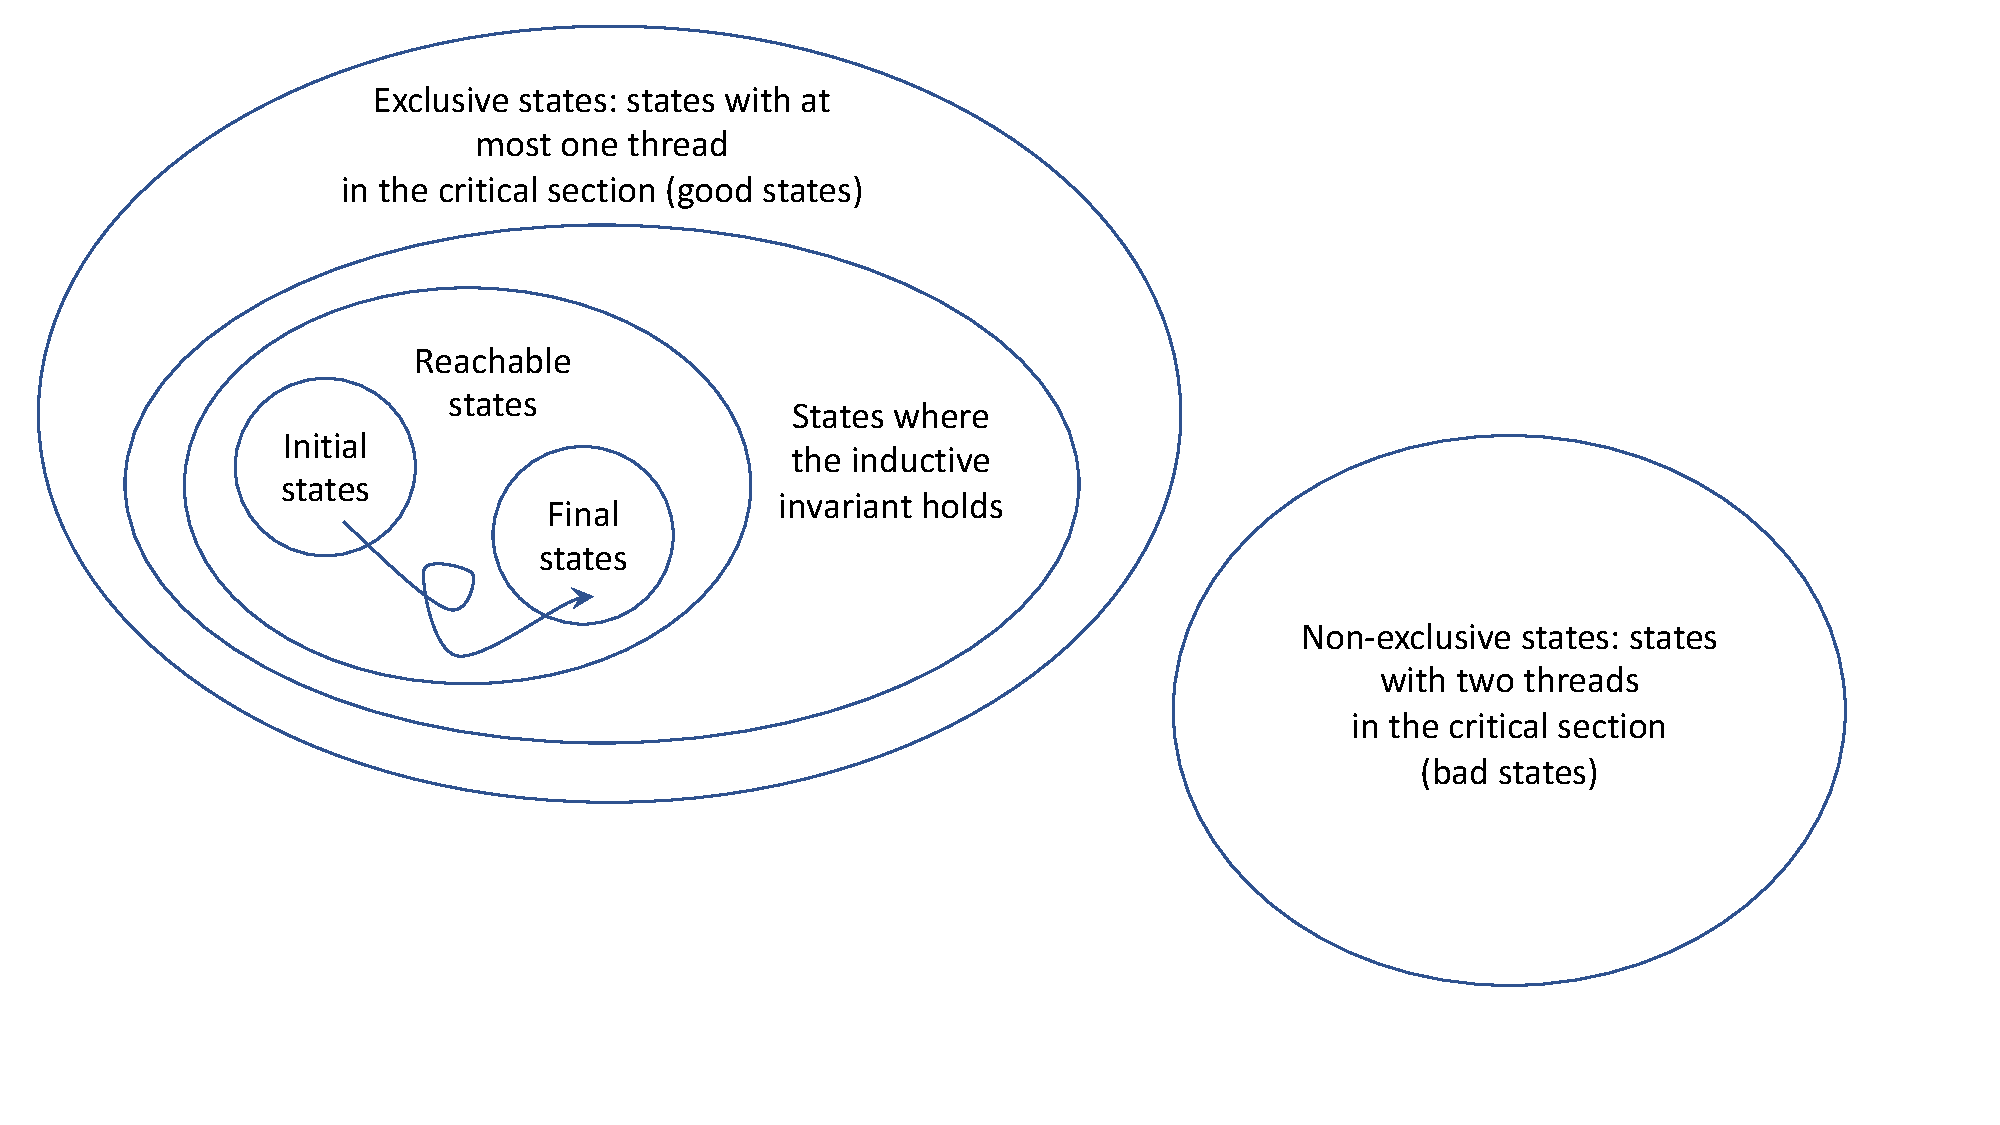
\includegraphics[width=6in]{figures/states-crop.pdf}
\end{center}
\caption{Venn diagram classifying all states and a trace.}
\label{fig:states}
\end{figure}

\glsadd{state}
\glsadd{process variable}
Why does it work?  We will focus here on how one might go about proving
mutual exclusion for an algorithm such as Peterson's.
For that, we have to understand a little bit more about how the CXL
machine works.
In Chapter~\ref{ch:cxlmachine} we talked about the concept of \emph{state}:
\index{state}
at any point in time the CVM is in a specific state.
A state is comprised of the values of the shared variables as well as
the values of the process variables
\index{process variable}
for each process, including its
program counter and the contents of its stack.
Everytime a process executes a CVM machine instruction, the
state changes (if only because the program counter of the process
changes).  We call that a \emph{step}.
\index{step}
Steps in CXL are atomic.
\glsadd{step}

\glsadd{trace}
The CVM starts in an initial state in which there is only
one process and its program counter is~0.  A \emph{trace}
\index{trace}
is a sequence of steps starting from the initial state.
When making a step, there are two sources of non-determinism
\index{non-determinism}
in CXL.
One is when
there is more than one process that can make a step.  The other is
when a process executes a \texttt{choose} operation and there is
more than one choice.
Because there is non-determinism, there are multiple possible traces.
We call a state \emph{reachable}
\index{reachable state}
if it is either the initial state
or it can be reached from the initial state through a trace.
A state is final
when there are no processes left to make state changes.

It is often useful to classify states into sets.
\emph{Initial}, \emph{final}, and \emph{reachable}, and \emph{unreachable}
are all examples of classes of states.
Figure~\ref{fig:states} depicts a Venn diagram of various classes of states
and a trace.
One way to classify states is to define a predicate over states.
All states in which \texttt{x = 1}, or all states where
there are two or more processes executing, are examples of such predicates.
For our purposes, it is useful to define a predicate that says that at
most one process is in the critical section.  We shall call such states
\emph{exclusive}.

An \emph{invariant} of a program
\index{invariant}
is a predicate that holds over all states that are reachable by that program.
We want to show that exclusivity is an invariant.
In other words, we want to show that the set of reachable states of executing
the program
is a subset of the set of states where there is at most one process in the critical
section.

One way to prove that a predicate is an invariant is through induction
on the number of steps.  First you prove that the predicate holds over
the initial state.  Then you prove that for every reachable state,
and for every step from that reachable state, the predicate also holds
over the resulting state.
For this you need a predicate that describes exactly which
states are reachable.
But we do not have such a predicate: we know how to describe the set
of reachable states, but given an arbitrary state it is not easy to
see whether it is reachable or not.

To solve this problem, we will use what is called an
\emph{inductive invariant}.
\index{inductive invariant}
An inductive invariant $I$ is a predicate over states that satisfies the following:
\begin{itemize}
\item $I$ holds in the initial state.
\item For any state in which $I$ holds and any process in the
state takes a step, then $I$ also holds in the resulting state.
\end{itemize}
Unlike an invariant, an inductive invariant must also hold over unreachable states.

One candidate for such an invariant is exclusivity itself.
After all, it certainly holds over the initial state.
And as CXL has already determined, exclusivity is an invariant:
it holds over every reachable state.
Unfortunately, it is not an \emph{inductive} invariant.
To see why, we need to consider an \emph{unreachable} state.
It is easy to construct one: let process~0 be at label \texttt{@cs}
and process~1 at the start of the \texttt{while} loop.
Also imagine that in this particular state $\mathtt{turn} = 1$.  Now let
process~1 make a sequence of steps.  Because $\mathtt{turn} = 1$,
process~1 will break out of the while loop and also enter the critical
section, entering a state that is not exclusive.
So exclusivity is an invariant, but not an inductive invariant.
Doing a inductive proof with an invariant that is not inductive is usually
much harder than doing one with an invariant that is.

\begin{figure}
\begin{code}
\VerbatimInput[xleftmargin=5mm,numbers=left]{code/PetersonInductive.cxl}
\end{code}
\caption{[PetersonInductive.cxl] Peterson's Algorithm with Inductive Invariant}
\label{fig:petersonproof}
\end{figure}

So we are looking for an inductive invariant that \emph{implies} exclusivity.
In other words, the set of states where the inducive invariant holds
must be a subset of the set of states where there is at most one process in
the critical section.
Let $C(i) = \mathtt{flags}[1 - i] \land
\mathtt{turn} = 1 - i$, that is, the condition on the \texttt{while} loop
for process~$i$.
Let predicate $I_p(i)$ be the following.
if process $i$ is at label \texttt{@cs} (i.e., process $i$ is in the critical section),
then $C(i)$ does not hold or process $1-i$ is executing after setting
$\mathtt{flags}[i]$ but still before setting \texttt{turn} to $1-i$.
More formally, $I_p(i) = \mathtt{process}(i)@cs) \Rightarrow (\lnot C(i) \lor \mathtt{process}(1-i)@gate)$.
For Peterson's Algorithm, an inductive invariant that works well is
$I_p(0) \land I_p(1)$.

Figure~\ref{fig:petersonproof} formalizes $I_p(i)$ in CXL.
The label \texttt{@gate} refers to the instruction that sets \texttt{turn} to $1-i$.
You can run Figure~\ref{fig:petersonproof} to determine
that $I_p(i)$ is indeed an invariant for $i = 0, 1$.

To see that the inductive invariant implies exclusivity, suppose not.  Then
when both process~0 and process~1 are in the critical section, the
following must hold:
$(\lnot C(0) \lor \mathtt{process}(1)@gate) \land
 (\lnot C(1) \lor \mathtt{process}(0)@gate)$.
We know that both flags are set.
We also know that neither process~0 nor process~1 is at label \texttt{@gate}
(because they are both at label \texttt{@cs}),
so this simplifies to $(\lnot C(0)) \land (\lnot C(1))$.
So we conclude that $\mathtt{turn} = 0 \land \mathtt{turn} = 1$, a
logical impossibility.  Thus $I_p(i)$ implies exclusivity.

To see that $I_p(0) \land I_p(1)$ is, in fact, an inductive invariant, first note that
it certainly holds in the initial state, because in the initial state no process
is in the critical section.
Without loss of generality, suppose $i=0$ (a benefit from the fact that the algorithm is
symmetric for both processes).  We still have to show that if we are in a state
in which $I_p(0)$ holds, then any step will result in a state in which
$I_p(0)$ still holds.
If $I_p(0)$ holds, process~0 is at label \texttt{@cs}.  If process~0
were to take a step, then in the next state process~0 would be no longer
at that label and $I_p(0)$ would hold trivially over the next state.
Therefore we only need to consider a step by process~1.

From $I_p(0)$ we know that one of the following three cases must hold before
process~1 takes a step:
\begin{enumerate}
\item \texttt{flags[1] = False};
\item \texttt{turn = 0};
\item process~1 is at label \texttt{@gate}.
\end{enumerate}

Let us consider each of these cases.
In the first case, if process~1 takes a step, there are two possibilities:
either $flags[1]$ will still be \texttt{False} (in which case the first case
continues to hold), or $flags[1]$ will be \texttt{True}
and process~1 will be at label \texttt{@gate} (in which case the third case
will hold).
We know that process~1 never sets \texttt{turn} to 1, so
if the second case holds before the step, it will also hold after the step.
Finally, if process~1 is at label \texttt{@gate} before the step, then after
the step \texttt{turn} will equal 0, and therefore the second case will hold
after the step.  qed.

We have now demonstrated mutual exclusion in Peterson's Algorithm in two
different ways: one by letting CXL explore all possible executions, the
other using an inductive invariant and proof by induction.  The former
is certainly easier, but it does not provide intuition for why the
algorithm works.  The second provides much more insight.  We therefore
encourage to include inductive invariants in your CXL code.

A cool anecdote is the following.  When the author of CXL had to teach
Peterson's Algorithm, he refreshed his memory by looking at the Wikipedia
page.  The page claimed that the following predicate is invariant:
if process $i$ is in the critical section, then $\lnot C(i)$ (i.e.,
$I_p(i)$ without the disjunct that process $1-i$ is at label \texttt{gate}).
To demonstrate that this predicate is not invariant, you can remove the
disjunct from Figure~\ref{fig:petersonproof} and run it to get a
counterexample.

This anecdote suggests the following.  If you need to do an induction
proof of an algorithm, you have to come up with an inductive invariant.
Before trying to prove the algorithm, you can check that the predicate is
at least invariant by testing it using CXL.  Doing so could potentially
avoid wasting your time on a proof that will not work because the
predicate is not invariant, and therefore not an inductive invariant either.
(The author fixed the Wikipedia page.)

\section*{Exercises}
\begin{problems}
\item Figure~\ref{fig:csonebit} presents another correct solution to the
mutual exclusion problem.  It is similar to the one in
Figure~\ref{fig:upflags}, but has a process \emph{back out and try again}
if it finds that the other process is either trying to enter the critical
section or already has.  Compare this algorithm with Peterson's.  What are
the advantages and disadvantages?
\item
Can you find an inductive invariant for the algorithm in
Figure~\ref{fig:csonebit} to prove it correct?
Here's a pseudo-code version of the algorithm to help you.  Each line
is an atomic action:
\begin{code}
\begin{verbatim}
    initially: flagX = flagY = False

    process X:                          process Y:
        X0: flagX = True                   Y0: flagY = True
        X1: if not flagY goto X4           Y1: if not flagX goto Y4
        X2: flagX = False                  Y2: flagY = False
        X3: goto X0                        Y3: goto Y0
        X4: ...critical section...         Y4: ...critical section...
        X5: flagX = False                  Y5: flagY = False
\end{verbatim}
\end{code}
\item A colleague of the author asked if the first two assignments in
Peterson's algorithm (setting \texttt{flags[self]})
to \texttt{True} and \texttt{turn} to \texttt{1 - self}) can be reversed.
After all, they are different variables assigned independent values---in a
sequential program one could surely swap the two assignments.
See if you can figure out for yourself if the two assignments can be
reversed.  Then run the program in Figure~\ref{fig:peterson} after reversing
the two assignments and describe in English what happens.
\item Bonus question:
Can you generalize Peterson's algorithm to more than two processes?
\end{problems}

\begin{figure}
\begin{code}
\VerbatimInput[xleftmargin=5mm,numbers=left]{code/csonebit.cxl}
\end{code}
\caption{[csonebit.cxl] Mutual exclusion using a flag per process.}
\label{fig:csonebit}
\end{figure}

\chapter{CXL Methods and Pointers}
\label{ch:method}
\index{CXL method}

A method \texttt{m} with argument \texttt{a} is invoked in its
most basic form as follows (assigning the result to~\texttt{r}).
\begin{code}
\begin{verbatim}
r = m a;
\end{verbatim}
\end{code}
That's right, no parentheses are required.  In fact, if you invoke
\texttt{m(a)}, the argument is \texttt{(a)}, which is the same
as \texttt{a}.
If you invoke \texttt{m()}, the argument is \texttt{()},
which is the empty tuple.
If you invoke \texttt{m(a, b)}, the argument is \texttt{(a, b)},
the tuple consisting of values \texttt{a} and \texttt{b}.

You may note that all this looks familiar.  Indeed, the syntax
is the same as that for dictionaries (see Chapter~\ref{ch:cxlmachine}).
Both dictionaries and methods map CXL values to CXL values,
and their syntax is indistinguishable.
If \texttt{f} is either a method or a
dictionary, and \texttt{x} is an arbitrary CXL value, then
\texttt{f x}, \texttt{f(x)}, and \texttt{f[x]} are all
the same expression in CXL.

\begin{figure}
\begin{code}
\VerbatimInput[xleftmargin=5mm,numbers=left]{code/PetersonMethod.cxl}
\end{code}
\caption{[PetersonMethod.cxl] Peterson's Algorithm accessed through methods.}
\label{fig:petersonmethods}
\end{figure}

CXL is not an object-oriented language like Python is.  In Python
you can pass a reference to an object to a method, and that method
can then update the object.  In CXL, it is also sometimes convenient
to have a method update a shared variable specified as an argument.
For this (as well as some other uses), CXL supports \emph{pointers}
\index{pointer}
to shared variables.
If \texttt{x} is a shared variable, then the expression \texttt{\&x}
 is a pointer to \texttt{x} (also known as the \emph{address}
\index{address}
of \texttt{x}).
Conversely, if \texttt{p} is a pointer to a shared variable, then the
expression \texttt{\^{}p} is the value of the shared variable.
In particular, \texttt{\^{}\&x == x}.
This is similar to how C pointers work.

Figure~\ref{fig:petersonmethods} again shows Peterson's algorithm,
but this time with methods defined to enter and exit the critical
section.
The name \texttt{mutex} is often used to denote a variable or value
that is used for mutual exclusion.
\texttt{P\_mutex} is a method that returns a ``mutex,'' which, in this
case, is a dictionary that contains Peterson's Algorithm's state:
a turn variable and two flags.
Both methods \texttt{P\_enter} and \texttt{P\_exit} take two arguments:
a pointer to a mutex and the process identifier (0 or 1).
\texttt{(\^{}pm).turn} is the value of the \texttt{.turn} key
in the mutex dictionary.  Note that the parentheses in this expression
are needed, as \texttt{\^{}pm.turn} would wrongly evaluate to
\texttt{\^{}(pm.turn)}.

You can put the first three methods in its own CXL source file
and include it using the CXL \texttt{import} statement.
\index{import statement}
\index{module}
This would
make the code re-usable by other applications.

For those who are
extra adventurous: you can add the \texttt{P\_enter} and
\texttt{P\_exit} methods to the \texttt{P\_mutex} dictionary
like so:
\begin{code}
\begin{verbatim}
dict{ .turn: 0, .flags: [ False, False ], .enter: P_enter, .exit: P_exit }
\end{verbatim}
\end{code}
That would allow you to simulate object methods.

\chapter{Spinlock}
\label{ch:spinlock}
\index{spinlock}
\glsadd{spinlock}

\begin{figure}
\begin{code}
\VerbatimInput[xleftmargin=5mm,numbers=left]{code/spinlock.cxl}
\end{code}
\caption{[spinlock.cxl] Mutual Exclusion using a ``spinlock'' based on test-and-set.}
\label{fig:tas}
\end{figure}

Figure~\ref{fig:uplock} showed a faulty attempt at solving mutual
exclusion using a lock.  The problem with the implementation of the
lock is that checking the lock and setting it if it is available is
not \emph{atomic}.  Thus multiple processes contending for the lock
can all ``grab the lock'' at the same time.  While Peterson's
algorithm gets around the problem, it is not efficient, especially
if generalized to multiple processes.  Instead, multi-core processors provide
so-called \emph{interlock instructions}:
\index{interlock instruction}
\glsadd{interlock instruction}
special machine instructions
that can read memory and then write it in an indivisible step.

While the CVM does not have any specific built-in interlock instructions,
it does have support for executing multiple instructions atomically.
This feature is available in the CXL language in two ways.
First, any CXL statement can be made atomic by placing a label in front
of it.  Second, a group of CXL statements can be made atomic
through its \texttt{atomic}
\index{atomic statement}
statement.
We can use \texttt{atomic} statement blocks to implement a wide variety of
interlock operations.
For example, we could fix the program in Figure~\ref{fig:inc} by
constructing an atomic increment operation for a counter, like so:
\begin{code}
\begin{Verbatim}[xleftmargin=5mm,numbers=left]
def atomic_inc(ptr):
    atomic:
        ^ptr = ^ptr + 1;
    ;
;
count = 0;
atomic_inc(&count);
\end{Verbatim}
\end{code}

Many CPUs have an atomic ``test-and-set'' (TAS)
\index{test-and-set}
\index{TAS}
operation.
Method \texttt{tas} in Figure~\ref{fig:tas} shows its specification.
Here \texttt{s} points to a shared boolean variable and \texttt{p}
to a private boolean variable, belonging to some process.
The operation copies the value of the shared variable to the
private variable (the ``test'')
and then sets the shared variable to \texttt{True} (``set'').

Figure~\ref{fig:tas} goes on how to implement mutual exclusion for
a set of $N$ processes.
The approach is called \emph{spinlock},
\index{spinlock}
because each process is ``spinning'' until
it can acquire the lock.
The program uses $N+1$ variables.
Variable \texttt{shared} is initialized to \texttt{False} while
\texttt{private[$i$]} for each process $i$ is initialized to \texttt{True}.
An important invariant, $I_1$, of the program is that at any time at most
one of these variables is \texttt{False}.
Another invariant, $I_2(i)$, is that if process $i$ is in the critical section,
then \texttt{private[$i$] == False}.
Between the two (i.e., $I_1 \land \forall i: I_2(i)$),
it is clear that only one process can be in the
critical section at the same time.

$I_1$ is an inductive invariant.
To see that invariant $I_1$ is maintained, note that
\texttt{\^{}p == True} upon entry of \texttt{tas}
(because of the condition on the \texttt{while} loop that the
\texttt{tas} method is invoked in).
So there are two cases:
\begin{enumerate}
\item \texttt{\^{}s} is \texttt{False} upon entry to \texttt{tas}.
Then upon exit \texttt{\^{}p == False} and \texttt{\^{}s == True}, maintaining
the invariant.
\item \texttt{\^{}s} is \texttt{True} upon entry to \texttt{tas}.
Then upon exit nothing has changed, maintaining the invariant.
\end{enumerate}
Invariant $I_1$ is also easy to verify for exiting the critical section.
Invariant $I_2(i)$ is obvious as (i) process $i$ only proceeds to the critical
section if \texttt{private[$i$] == False}, and (ii) no other process modifies
\texttt{private[$i$]}.

\begin{figure}
\begin{code}
\VerbatimInput[xleftmargin=5mm,numbers=left]{code/spinlockInv.cxl}
\end{code}
\caption{[spinlockInv.cxl] Checking invariants.}
\label{fig:tasinv}
\end{figure}

CXL can check these invariants as well.  Figure~\ref{fig:tas} already
has the code to check $I_2(i)$.  But how would one go about checking an
invariant like $I_1$?  Invariants must hold for every state.
For $I_2$ we only need an assertion at label \texttt{@cs} because the
premisse is that there is a process at that label.  However, we would
like to check $I_1$ in \emph{every state} (after the variables have
been initialized).

We can do this by adding another process that, in a loop,
checks the invariant.  Figure~\ref{fig:tasinv} shows the code.
Method \texttt{checkInvariant()} checks to see if the invariant holds
in a state.  It introduces a new feature of CXL: the ability to have
variables local to a method.  In this case, the process variable \texttt{sum}
is used to compute the number of shared variables that have value
\texttt{False}.
The function is invoked by in a loop by a process that runs alongside
the other processes.
In CXL, \texttt{assert} statements are executed atomically, so the
evaluation of the assertion is not interleaved with the execution
of other processes.
Because CXL tries every possible execution, the process is guaranteed
to find violations of the invariant if it does not hold.

\section*{Exercises}
\begin{problems}
\item Implement an atomic swap operation.  It should take two pointer arguments
and swap the values.
\item Implement a spinlock using the atomic swap operation.
\item Write out the invariants that need to hold and check them using CXL.
\end{problems}

\chapter{Locks and Blocking}
\label{ch:synch}
\index{lock}
\index{synch module}

\begin{figure}
\begin{code}
\VerbatimInput[xleftmargin=5mm,numbers=left]{code/csTAS.cxl}
\end{code}
\caption{[csTAS.cxl] Fixed version of Figure~\ref{fig:uplock} using test-and-set.}
\label{fig:tas2}
\end{figure}

In Figure~\ref{fig:tas} we have shown a solution based on a shared
variable and a private variable for each process.   The private
variables themselves are actually implemented as shared variables,
but they are accessed only by their respective processes.
There is no need to keep \texttt{private} as a shared
variable---we only did so to be able to show and check the invariants.
Figure~\ref{fig:tas2} shows a more straightforward implementation of spinlock.
The solution is similar to the na\"{i}ve solution of Figure~\ref{fig:uplock},
but uses test-and-set to check and set the lock variable atomically.
This approach is general for any number of processes.

It is important to appreciate the difference between an
\emph{atomic section} (the statements executed within an
\texttt{atomic} statement) and a \emph{critical section}
(protected by a lock of some sort).
The former ensures that while the
atomic statement is executing no other process can execute.
The latter allows multiple processes to run concurrently,
just not within the critical section.
The former is rarely available to a programmer, while the latter
is very common.

In CXL, atomic statements allow you to \emph{implement} your own
synchronization primitives like test-and-set.  Other common examples
include compare-and swap and fetch-and-add.  Atomic statements
are not intended to \emph{replace} locks or other synchonization primitives.
When solving synchronization problems you should not directly use
atomic statement but use the synchronization primitives that are available
to you.  But if you want to design a new synchronization primitive, then
use \texttt{atomic} by all means.

\begin{figure}
\begin{code}
\begin{Verbatim}[xleftmargin=5mm,numbers=left]
def tas(lk):
    atomic:
        result = ^lk;
        ^lk = True;
    ;
;
def Lock():
    result = False;
;
def lock(lk):
    while tas(lk):
        pass;
    ;
;
def unlock(lk):
    ^lk = False;
;
\end{Verbatim}
\end{code}
\caption{The \texttt{Lock} interface in the \texttt{synch} module.}
\label{fig:spinlocks}
\end{figure}

\begin{figure}
\begin{code}
\VerbatimInput[xleftmargin=5mm,numbers=left]{code/UpLock.cxl}
\end{code}
\caption{[UpLock.cxl] Program of Figure~\ref{fig:inc} fixed with a lock.}
\label{fig:incfixed}
\end{figure}

Locks are probably the most prevalent and basic form of synchronization
in concurrent programs.  For this reason, CXL has a module called
\texttt{synch} that includes support for locks.
Figure~\ref{fig:spinlocks} shows how they are implemented, and
Figure~\ref{fig:incfixed} gives an example of how they may be used,
in this case to fix the program of Figure~\ref{fig:inc}.
Notice that the module completely hides the implementation of the
lock.
The \texttt{synch} module includes a variety of other useful
synchronization primitives, which will be discussed in later
chapters.

\glsadd{blocked process}
We call a process \emph{blocked}
\index{blocked process}
in a state if the process is waiting on a low-level synchronization
variable and cannot make progress without the help of another process.
A process trying to
acquire a test-and-set spinlock held by another process is a good example
of a process being blocked.
The only way forward is if the other process releases the lock.

\begin{figure}
\begin{code}
\begin{Verbatim}[xleftmargin=5mm,numbers=left]
import list;

def Lock():
    result = dict{ .locked: False, .suspended: [] };
;
def lock(lk):
    atomic:
        if (^lk).locked:
            stop (^lk).suspended;
            assert (^lk).locked;
        else:
            (^lk).locked = True;
        ;
    ;
;
def unlock(lk):
    atomic:
        if (^lk).suspended == []:
            (^lk).locked = False;
        else:
            go (head((^lk).suspended)) ();
            (^lk).suspended = tail((^lk).suspended);
        ;
    ;
;
\end{Verbatim}
\end{code}
\caption{The \texttt{Lock} interface in the \texttt{synchS} module uses suspension.}
\label{fig:suspension}
\end{figure}

In most operating systems, processes are virtual and can be suspended
until some condition changes.  For example, a process can be suspended
until the lock is available to it.
In CXL, a process can suspend itself and save its context (state) in a
list.  Recall that the context of a process consists of its name tag,
its program counter, and the contents of its register and stack.
A context is a regular CXL value.
The syntax of the expression is as follows:

\begin{code}
\begin{verbatim}
stop L
\end{verbatim}
\end{code}

Here \texttt{L} is a shared list.
Another process can revive the process using the \texttt{go}
\index{go statement}
statement:

\begin{code}
\begin{verbatim}
go C R
\end{verbatim}
\end{code}

Here \texttt{C} is a context and \texttt{R} is a CXL value.
It causes a process with context \texttt{C} to be added to the state that has
just executed the \texttt{stop}
\index{stop expression}
expression.  The \texttt{stop} expression returns the value \texttt{R}.

There is a second version of the \texttt{synch} module that uses suspension
instead of spinlocks.
Figure~\ref{fig:suspension} shows the same \texttt{Lock} interface implemented
using suspension.
The interface is implemented as follows:
\begin{itemize}
\item A \texttt{Lock} maintains both a boolean indicating whether the
lock is taken and a list of contexts of processes that want to acquire the lock.
\item
\texttt{lock} sets the lock if available and suspends itself if not.
Note that \texttt{stop} is called within an \texttt{atomic} statement---this is
the only exception to an atomic statement running to completion.  While the
process is running no other processes can run, but when it suspends itself
it allows other processes to run.
\item
\texttt{unlock} checks to see if any processes are waiting to get the lock.
If so, it uses the \texttt{head} and \texttt{tail}
methods from the \texttt{list} module (see Appendix~\ref{ap:module})
to resume the first process that got
suspended and to remove its context from the list.
\end{itemize}
Selecting the first process is a design choice.  Another implementation could
have picked the last one, and yet another implementation could have used
\texttt{choose} to pick an arbitrary one.  Selecting the first is a common
choice in lock implementations as it prevents \emph{starvation}:
\index{starvation}
every process
gets a chance to obtain the lock (assuming every process eventually releases
it).  Chapter~\ref{ch:starvation} will talk more about starvation and how
to prevent it.

CXL allows you to select which version of the \texttt{synch} module you would
like to use with the \texttt{-m} flag.
\index{module}
For example,

\begin{code}
\begin{verbatim}
cxl -m synch=synchS x.cxl
\end{verbatim}
\end{code}

runs the file \texttt{x.cxl} using the suspension version of the \texttt{synch} module.
You will find that using the \texttt{synchS} module often leads to searching a
significantly larger search space than using the \texttt{synch} module.
Part of the reason is that the \texttt{synchS} module keeps track of the order
in which processes wait for a lock.

\section*{Exercises}
\begin{problems}
\item Write a synchronization module using your own implementation of \texttt{Lock}
(for example, using Peterson's algorithm or using \texttt{swap}).
\item
Run Figure~\ref{fig:incfixed} using (1) \texttt{synch}, (2), \texttt{synchS},
and (3) your own module.  Report how many states were explored by CXL for each
version of the module.
\end{problems}

\chapter{Reader/Writer Locks using Busy Waiting}
\label{ch:rdwrbusy}
\index{reader/writer lock}
\glsadd{reader/writer lock}

\begin{figure}
\begin{code}
\VerbatimInput[xleftmargin=5mm,numbers=left]{code/RWbusy.cxl}
\end{code}
\caption{[RWbusy.cxl] Busy-Waiting Reader/Writer Lock implementation.}
\label{fig:rwbusy}
\end{figure}

\begin{figure}
\begin{code}
\VerbatimInput[xleftmargin=5mm,numbers=left]{code/RWbusytest.cxl}
\end{code}
\caption{[RWbusytest.cxl] Test code for Figure~\ref{fig:rwbusy}.}
\label{fig:rwbusytest}
\end{figure}

\begin{figure}
\begin{center}
\includegraphics[width=2.5in]{figures/rdwr-crop.pdf}
\end{center}
\caption{High-level state diagram specification of reader/writer locks with
up to two processes.
The first number in a state gives the number of processes; the second number is the
number of processes reading in the critical section; the third is the number of
processes writing in the critical section.}
\label{fig:rdwr}
\end{figure}

Locks are useful when accessing a shared data structure.  By preventing
more than one process from accessing the data structure at the same
time, conflicting accesses are avoided.  However, not all concurrent
accesses conflict, and opportunities for concurrency may be lost,
hurting performance.  One important case is when multiple processes
are simply reading the data structure.
In many applications, reads are the majority of all accesses.
Allowing reads to proceed concurrently can significantly improve performance.

What we want is a special kind of lock that allows either one writer
or one or more readers to be in the critical section.  This is called
a \emph{reader/writer lock}~\cite{CHP71}.
We will explore various ways of implementing reader/writer locks in
this chapter and future ones.

Figure~\ref{fig:rwbusy} presents a solution that uses a
single (ordinary) lock and two counters: one that maintains the number
of readers and one that maintains the number of writers.
Figure~\ref{fig:rwbusytest} shows how the code may be used.
We will call the lock the \emph{mutex} to distinguish it clearly from
the reader/writer lock that we are implementing.
The mutex is used to protect shared access to the counters.
The program shows a process that executes in a loop.
Each time, it decides whether to read or write.
The critical section is spread between two labels:
readers access \texttt{@rcs} and writers access \texttt{@wcs}.
The specification is that if a reader is at label \texttt{@rcs},
no writer is allowed to be at label \texttt{@wcs}.  Vice versa, if
a writer is at label \texttt{@wcs}, no reader is allowed to be at
label \texttt{@rcs} \emph{and} there cannot be another writer at
label \texttt{@wcs}.  Figure~\ref{fig:rdwr} shows a high-level
specification for two processes.

A process that wants to read first waits until there are no writers:
\texttt{nwriters == 0}.  Then it increments the number of readers.
Similarly, a
process that wants to write waits until there are no readers \emph{or} writers.
Then it increments the number of writers.
The important invariants in this code are:
\begin{itemize}
\item $n$ readers at \texttt{@rcs} $\Rightarrow \mathtt{nreaders} \ge n$,
\item $n$ writers at \texttt{@wcs} $\Rightarrow \mathtt{nwriters} \ge n$,
\item $(\mathtt{nreaders} \ge 0 \land \mathtt{nwriters} = 0) \lor
    (\mathtt{nreaders} = 0 \land 0 \le \mathtt{nwriters} \le 1)$.
\end{itemize}
It is easy to see that the invariants hold and imply the reader/writer
specification.
The solution also supports progress: if no process is in the critical
section then any process can enter.  Better still: if any reader is in the
critical section, any other reader is also able to enter.

\begin{figure}
\begin{code}
\VerbatimInput[xleftmargin=5mm,numbers=left]{code/RWbusychk.cxl}
\end{code}
\caption{[RWbusychk.cxl] Checking for Busy Waiting.}
\label{fig:rwblock}
\end{figure}

\glsadd{busy waiting}
While correct, it is not considered a good solution.
The solution is an example of what is called \emph{busy-waiting}
\index{busy waiting}
(aka \emph{spin-waiting}):
\index{spin waiting}
processes spin in a loop until some desirable application-level condition is met.
Figure~\ref{fig:inc} also has an example of busy-waiting: the \texttt{main}
process waits for the other two processes to finish by checking their \texttt{done}
flags.

The astute reader might wonder if obtaining the mutex itself is an
example of busy-waiting.  After all, the CXL \texttt{synch} implementation
of \texttt{lock()} spins in a loop until the mutex is available
(see Figure~\ref{fig:spinlocks}).
However, there is a big difference.  As we pointed out, the processes that
are waiting for a spinlock are \emph{blocked}.
In most operating systems and programming language runtimes,
when a process acquires a mutex, the process is placed on a scheduling
queue and stops using CPU cycles until the mutex becomes available.
CXL supports this with the \texttt{synchS} module.
Busy waiting disables all this: even when using the \texttt{synchS}
module, readers and writers only get suspended temporarily in case
there is contention for the mutex.
A process trying to obtain a read or write lock in
Figure~\ref{fig:rwbusy} has to obtain the mutex repeatedly
until the read or write lock is available.

Thus, it is considered ok to have processes be blocked while waiting
for application-specific conditions, but not for them to
busy-wait for application-specific conditions.

CXL does not complain about Figure~\ref{fig:rwbusy}, but, using
the right test, CXL can be used to check for busy-waiting.
Figure~\ref{fig:rwblock} presents such a test.
Note that the initialization code obtains a read lock, preventing
all readers and writers from entering the critical section.
In that case, those processes should ideally be blocked and CXL
can test for that by running it with the \texttt{-b} flag.
This flag tells CXL to check
that all states are non-terminating and lead to a state in which
all processes are blocked.

\section*{Exercises}
\begin{problems}
\item Draw additional states and steps in Figure~\ref{fig:rdwr}
for three processes.
\item Using busy waiting, implement a ``bound lock'' that allows
up to \texttt{M} processes to acquire it at the same time.  A bound lock
with \texttt{M == 1} is an ordinary lock.
You should define a constant \texttt{M} and two methods:
\texttt{acquire\_bound\_lock()}
and \texttt{release\_bound\_lock()}.
\item Write a test program for your bound lock
that checks that no more than \texttt{M} processes can acquire the
bound lock.
\end{problems}

\chapter{Reader/Writer Locks with Blocking}
\label{ch:rdwr2}

\begin{figure}
\begin{code}
\VerbatimInput[xleftmargin=5mm,numbers=left]{code/RWlock.cxl}
\end{code}
\caption{[RWlock.cxl] Reader/Writer with Two Locks.}
\label{fig:rw2lock}
\end{figure}

\begin{figure}
\begin{code}
\VerbatimInput[xleftmargin=5mm,numbers=left]{code/RWmulti.cxl}
\end{code}
\caption{[RWmulti.cxl] Checking that multiple readers can acquire the read lock.}
\label{fig:rwmulti}
\end{figure}

Figure~\ref{fig:rw2lock} presents a reader/writer lock implementation
that does not busy-wait.
It uses two ordinary locks: \texttt{rwlock} is used by both readers and writers,
while \texttt{rlock} is only used by readers.
\texttt{rwlock} is held either when readers are at label \texttt{@rcs}
or when a writer is at label \texttt{@wcs}.
\texttt{rlock} is used to protect the \texttt{nreaders} variable that
counts the number of readers in the critical section. 

The invariants that imply the reader/writer specification
(which are again easy to verify) are as follows:

\begin{itemize}
\item $n$ readers at \texttt{@rcs} $\Rightarrow \mathtt{nreaders} \ge n$,
\item $\exists$ writer at \texttt{@wcs} $\Rightarrow \mathtt{nreaders} = 0$,
\end{itemize}

A writer simply acquires \texttt{rwlock} to enter the critical section
and releases it to exit.  The \emph{first} reader to enter the critical
section acquires \texttt{rwlock} and the \emph{last} reader to exit
the critical section releases \texttt{rwlock}.
The implementation satisfies progress: if no process is in the critical
section than any process enter.

It is instructive to see what happens when a writer is in the critical
section and two readers try to enter.  The first reader successfully
acquires \texttt{rlock} and but blocks when trying to acquire
\texttt{rwlock}, which is held by the writer.  The second reader blocks
trying acquire \texttt{rlock} because it is held by the first reader.
When the writer leaves the critical section, the first reader acquires
\texttt{rwlock}, sets \texttt{nreaders} to 1, and releases \texttt{rlock}.
\texttt{rwlock} is still held.
Then the second reader acquires \texttt{rlock} and, assuming the first
reader is still in the critical section, increments \texttt{nreaders} to 2
and enters the critical section \emph{without} acquiring \texttt{rwlock}.
\texttt{rwlock} is essentially jointly held by both readers.
It does not matter in which order they leave: the second will release
\texttt{rwlock}.

While CXL does not detect any issues, we must remember what it is checking
for: it checks to make sure that there are never a reader and a writer
in the critical section, and there are never two readers in the critical
section.  Moreover, it checks progress: all executions eventually terminate.
What it does \emph{not} check is if the code allows more than one reader
in the critical section.  Indeed, we could have implemented the reader/writer
lock as in Figure~\ref{fig:rwmulti} using an ordinary lock, never allowing
more than one process in the critical section.

Figure~\ref{fig:rwmulti} contains a new test that ensures that indeed more
than one reader can enter the critical section at a time.  It does so by
having processes sometimes wait in the critical section until all other readers
are there.  If other readers cannot enter, then that process enters in an
infinite loop that CXL will readily detect.  Try it out!

An important lesson here is that one should not celebrate too early if CXL
does not find any issues.  While a test may be successful, a test may not
explore all desirable executions.  While CXL can help explore all cornercases
in a test, it cannot find problems that the test is not looking for.

\section*{Exercises}
\begin{problems}
\item Why do you suppose the code in Figure~\ref{fig:rwmulti} uses a flag
per process rather than a simple counter?
Can you write a version of this test that uses a counter instead
of a flag per process?
% \item Write a ``library implementation'' of reader/writer locks so multiple
% reader/writer locks can be instantiated.
\item Write a test program for ``bound locks'' (as implemented in the
exercises of the last chapter) that checks that up to \texttt{M} processes
can acquire the bound lock at the same time.
\item It can be useful for a process to \emph{downgrade} its write lock
to a read lock when its done writing but not done reading.  Implement
\texttt{downgrade}.  Note, you cannot do this simply by releasing the
write lock and then obtaining the read lock.
\end{problems}

\chapter{Semaphores}
\label{ch:semaphore}
\index{semaphore}
\glsadd{semaphore}

\begin{figure}
\begin{code}
\begin{Verbatim}[xleftmargin=5mm,numbers=left]
def Semaphore(cnt):
    result = cnt;
;
def P(sema):
    let blocked = True:
        while blocked:
            atomic:
                if (^sema) > 0:
                    ^sema = (^sema) - 1;
                    blocked = False;
                ;
            ;
        ;
    ;
;
def V(sema):
    atomic:
        ^sema = (^sema) + 1;
    ;
;
\end{Verbatim}
\end{code}
\caption{The \texttt{Semaphore} interface in the \texttt{synch} module.}
\label{fig:semaphore}
\end{figure}

\begin{figure}
\begin{code}
\VerbatimInput[xleftmargin=5mm,numbers=left]{code/DinersSema.cxl}
\end{code}
\caption{[DinersSema.cxl] Italian Philosophers.}
\label{fig:dinerssema}
\end{figure}

So far we have looked at how to protect a single resource.
Some types of resources may have multiple units.
If there are only $n$ units, no more than $n$ units can be used at a time;
if all are in use and a process comes along that needs one of the units,
it has to wait until another process releases one of the units.
Note that we cannot solve this problem simply using a lock per unit---allocating
a unit requires access to the entire collection.

Consider a variant of the Dining Philosophers (which were clearly Dutch---who
else need two forks to eat a meal?) that we call Italian Philosophers (who only
use one fork each to eat spaghetti---they need the other to speak\footnote{The joke
was provided to me by my dear friend and colleague Lorenzo Alvisi.}).
Again, there are five philosophers.
This time, however, there is a glass sitting in the middle of the table with only
three forks in it.  A philosopher needs one of those forks to eat, but clearly,
no more than three philosophers can eat at a time.
See if you can come up with a deadlock-free solution using locks.  Represent
each fork as a lock.  It's not easy.
It is not hard to come up with a solution that uses a single lock
and busy waiting, but we would like to avoid busy waiting.

Introduced by Dijkstra,
a \emph{semaphore} is a synchronization primitive that fits the bill~\cite{EWD35}.
A semaphore is essentially
a counter that can be incremented and decremented but is not allowed to go
below zero.  The semaphore counter is typically initialized to the number of
units of a resource initially available.
When allocating a resource, a process decrements the
counter using the \texttt{P}
\index{P}
\index{Procure}
operation.  You can think of \texttt{P} standing
for \emph{Procure}, as in procuring the resource associated with the semaphore.
The \texttt{P} operation blocks the invoking process if the counter is zero.
To release the resource, a process increments the resource using the
\texttt{V}
\index{V}
\index{Vacate}
operation.  You can think of \texttt{V} standing for \emph{vacate},
as in vacating the resource.
One can think of a semaphore as a generalization of a lock.  In fact, a
lock can be implemented by a semaphore initialized to 1.  Then \texttt{P}
procures the lock, and \texttt{V} vacates the lock.

Figure~\ref{fig:semaphore} shows the \texttt{synch} module implementation of
semaphores.
It represents a semaphore as an integer.
Figure~\ref{fig:dinerssema} shows a solution to the Italian Philosphers problem
using a semaphore.

You may find the free ``The Little Book of Semaphores'' by
Allen Downey a great resource for working with semaphores~\cite{Downey09}.

\section*{Exercices}
\begin{problems}
\item Add an assertion that demonstrates that at most three
Italian philosophers are eating at the same time?
\item Implement a test program that checks to see that
the solution allows more than one Italian philosopher to eat at the same time?
\item \label{ex:qsort}
Figure~\ref{fig:qsort} shows an iterative implementation of the Qsort
algorithm, and Figure~\ref{fig:qsorttest} an accompanying test program.
The array to be sorted is stored in  shared variable \texttt{a}.
Another shared variable, \texttt{todo}, contains the ranges of the
array that need to be sorted (initially the entire array).
Re-using as much of this code as you can, implement a parallel version of
this.  You should not have to change the methods \texttt{swap}, \texttt{partition},
or \texttt{sortrange} for this.  Create \texttt{NWORKERS} ``worker processes''
that should replace the \texttt{qsort} code.  Each worker loops until \texttt{todo}
is empty and sorts the ranges that it finds until then.  The \texttt{main}
process needs to wait until all workers are done.  Use a semaphore for this:
the \texttt{main} process should use \texttt{P} to wait for each
worker to terminate.  After that it should check that the array is sorted and
that it is a permutation of the original array.
\end{problems}

\begin{figure}
\begin{code}
\VerbatimInput[xleftmargin=5mm,numbers=left]{code/qsort.cxl}
\end{code}
\caption{[qsort.cxl] Iterative qsort() implementation.}
\label{fig:qsort}
\end{figure}

\begin{figure}
\begin{code}
\VerbatimInput[xleftmargin=5mm,numbers=left]{code/qsorttest.cxl}
\end{code}
\caption{[qsorttest.cxl] Test program for Figure~\ref{fig:qsort}.}
\label{fig:qsorttest}
\end{figure}

\chapter{Bounded Buffer}
\label{ch:bb}
\index{bounded buffer}
\index{producer/consumer problem}
\glsadd{producer/consumer problem}

\begin{figure}
\begin{center}
\includegraphics[width=2.5in]{figures/pc-crop.pdf}
\end{center}
\caption{High-level state diagram specification of producers/consumers.}
\label{fig:pc}
\end{figure}

\begin{figure}
\begin{code}
\VerbatimInput[xleftmargin=5mm,numbers=left]{code/BBsema.cxl}
\end{code}
\caption{[BBsema.cxl] Bounded Buffer implementation using semaphores.}
\label{fig:boundedbuffer}
\end{figure}

\begin{figure}
\begin{code}
\begin{verbatim}
cxl -b -c NSLOTS=0 -c NPRODS=1 -c NCONSS=1 PCsema.cxl
cxl -b -c NSLOTS=1 -c NPRODS=0 -c NCONSS=1 PCsema.cxl
cxl    -c NSLOTS=1 -c NPRODS=1 -c NCONSS=0 PCsema.cxl
cxl    -c NSLOTS=1 -c NPRODS=1 -c NCONSS=1 PCsema.cxl
cxl -b -c NSLOTS=1 -c NPRODS=1 -c NCONSS=2 PCsema.cxl
cxl -b -c NSLOTS=1 -c NPRODS=2 -c NCONSS=0 PCsema.cxl
cxl    -c NSLOTS=1 -c NPRODS=2 -c NCONSS=1 PCsema.cxl
cxl    -c NSLOTS=1 -c NPRODS=2 -c NCONSS=2 PCsema.cxl
cxl -b -c NSLOTS=1 -c NPRODS=2 -c NCONSS=3 PCsema.cxl
cxl    -c NSLOTS=2 -c NPRODS=1 -c NCONSS=0 PCsema.cxl
cxl    -c NSLOTS=2 -c NPRODS=1 -c NCONSS=1 PCsema.cxl
cxl -b -c NSLOTS=2 -c NPRODS=1 -c NCONSS=2 PCsema.cxl
cxl    -c NSLOTS=2 -c NPRODS=2 -c NCONSS=0 PCsema.cxl
cxl    -c NSLOTS=2 -c NPRODS=2 -c NCONSS=1 PCsema.cxl
cxl    -c NSLOTS=2 -c NPRODS=2 -c NCONSS=2 PCsema.cxl
cxl -b -c NSLOTS=2 -c NPRODS=2 -c NCONSS=3 PCsema.cxl
cxl -b -c NSLOTS=2 -c NPRODS=3 -c NCONSS=0 PCsema.cxl
cxl    -c NSLOTS=2 -c NPRODS=3 -c NCONSS=1 PCsema.cxl
cxl    -c NSLOTS=2 -c NPRODS=3 -c NCONSS=2 PCsema.cxl
cxl    -c NSLOTS=2 -c NPRODS=3 -c NCONSS=3 PCsema.cxl
\end{verbatim}
\end{code}
\caption{Script for testing producer/consumer synchronization
(assuming the code is in file \texttt{PCsema.cxl}).}
\label{fig:pcscript}
\end{figure}

A good example of a resource with multiple units is the
so-called \emph{bounded buffer} (aka \emph{ring buffer}).
\index{ring buffer}
Suppose you have a \emph{producer} (some process) wanting to
communicate a stream of items with a \emph{consumer} (another process).
A bounded buffer is essentially
a queue implemented using a circular buffer
\index{circular buffer}
of a certain length and two pointers:
one where the producer inserts items, and one where the consumer extracts
items.  If the
buffer is full, the producer must wait; if the buffer is empty, the
consumer must wait.
This problem is known as the ``Producer/Consumer Problem'' and was
proposed by Dijkstra~\cite{EWD329}.

The producer/consumer pattern is common.  Processes may be arranged
in \emph{pipelines},
\index{pipeline}
where each upstream process is a producer and each downstream
process is a consumer.
Or processes may be arranged in a manager/worker pattern, with a manager
producing jobs and workers executing them in parallel.

In general, we allow multiple producers and multiple consumers
all sharing the same bounded buffer.
Figure~\ref{fig:pc} gives a high-level description.  The
two numbers in a state specify
the number of items that the producers still can produce and
the number of items that the consumers have consumed.  In this case
there are three items to produce initially.

\begin{figure}
\begin{code}
\VerbatimInput[xleftmargin=5mm,numbers=left]{code/BBsemadata.cxl}
\end{code}
\caption{[BBsemadata.cxl] Test whether the bounded buffer delivers the right data in the
right order.}
\label{fig:PCsemadata}
\end{figure}

Figure~\ref{fig:boundedbuffer} presents the implementation of a bounded
buffer using semaphores.  It features a circular bounded buffer \texttt{buf} with
slots numbered 1 through \texttt{NSLOTS}.  There are two indexes into
the buffer: \texttt{b\_in} specifies where the next produced item is inserted,
while \texttt{b\_out} specifies from where the next can be consumed.
As there may be multiple producers and multiple
consumers, updates to the indexes, which are shared variables, must be protected.
To this end, we use two semaphores as locks: \texttt{l\_in} for \texttt{b\_in}
and \texttt{l\_out} for \texttt{b\_out}.

Without additional synchronization, the indexes may overflow and point to invalid
entries in the circular buffer.
For this, there is a semaphore \texttt{n\_full} that
keeps track of the number of filled entries in the buffer and a semaphore
\texttt{n\_empty} that keeps track of the number of empty entries in the buffer.

To add an item to the bounded buffer (\texttt{produce(item)}), the producing
process first has to wait until there is room in the bounded buffer.
To this end, it invokes \texttt{P(n\_empty)}, which waits until
\texttt{n\_empty > 0} and atomically decrements \texttt{n\_empty} once this
is the case.  In other words, the producer procures an empty slot.
Next, it adds the item to the next position in the buffer.
Since there may be more than one empty slot, multiple producers may attempt
to do the same thing concurrently.  Hence the use of the \texttt{l\_in}
semaphore used as a lock.  Finally, once the item is added, the process
increments the \texttt{n\_full} semaphore to signal to consumers that
an item is available.
The consumer code is symmetric.

Note the quite different usage of the \texttt{l\_} semaphores and \texttt{n\_}
semaphores.
People often call semaphores that are used as locks \emph{binary semaphores},
\index{binary semaphore}
as they only take on the values 0 and 1.
They protect critical sections.
The second type of semaphores are called \emph{counting semaphores}.
\index{counting semaphore}
They can be used to send signals between processes.
However, binary and counting semaphores are implemented the same way.

We can run the code through CXL, but what would it test?  There are no
assert statements in the code.
We can split the functionality of this code into two pieces.  One is
the synchronization part: producers should never run more than \texttt{NSLOTS}
ahead of the consumers, but they should be able to produce up to \texttt{NSLOTS}
items even if there are no consumers.  The other part is the data: we want
to make sure that the items are sent through the buffer in order and without
loss.  We will first focus on the synchronization.

The first part can be tested with the code given in Figure~\ref{fig:pc}, by
experimenting with different non-negative values for the three constants.
In particular, any run with a positive \texttt{NSLOTS} and
$\mathtt{NCONSS} \le \mathtt{NPRODS} \le \mathtt{NCONSS} + \mathtt{NSLOTS}$
should terminate, while other values should lead to processes blocking.
To this this, one can write a script like the one in Figure~\ref{fig:pcscript}.

Figure~\ref{fig:PCsemadata} tests whether the correct data is sent in
the correct order.  There are the same number of producers and consumers.
Each producer $i$ produces two tuples: $(i, 0)$ and $(i, 1)$ in that order.
Each consumer consumes two tuples and checks that the tuples are different
and that, if the two tuples come from the same producer, then they have to
be in the order sent.
Moreover, consumers add the tuples they received to the set
\texttt{received} (atomically---a lock could have been used here as well).)
The \texttt{main()} process waits for all consumers to have received
exactly the set of tuples that the producers produce.

\section*{Exercises}
\begin{problems}
\item Change the code in Figure~\ref{fig:boundedbuffer} so that
\texttt{produce()} fails if the buffer is full rather than block.
\texttt{produce()} should return \texttt{False} if it fails
and return \texttt{True} if it succeeds.
\item Implement a \emph{bounded stack}.  Method \texttt{push(item)}
should block if the stack is full.  Method \texttt{pop()} should block
until the stack is non-empty and then return an item.
\item \label{ex:gpu} Implement a thread-safe GPU allocator by modifying
Figure~\ref{fig:gpu}.
There are \texttt{N} GPUs identified by the numbers
1 through \texttt{N}.  Method \texttt{gpuAlloc()} returns the identifier
of an available GPU, blocking if there is currently no available GPU.
Method \texttt{gpuRelease(gpu)} releases the given GPU.  It never needs
to block.
\end{problems}

\begin{figure}
\begin{code}
\VerbatimInput[xleftmargin=5mm,numbers=left]{code/gpu.cxl}
\end{code}
\caption{[gpu.cxl] A thread-unsafe GPU allocator.}
\label{fig:gpu}
\end{figure}

\chapter{Split Binary Semaphores}
\label{ch:sbs}
\index{split binary semaphore}

\begin{figure}
\begin{code}
\VerbatimInput[xleftmargin=5mm,numbers=left]{code/RWsbs.cxl}
\end{code}
\caption{[RWsbs.cxl] Reader/Writer Lock implementation using Split Binary Semaphores.}
\label{fig:RWsplitsema}
\end{figure}

Reader/writer locks and bounded buffers are both examples of what are
sometimes called \emph{conditional critical sections}
\index{conditional critical section}
(CCSs)~\cite{Hoare73}.
\glsadd{conditional critical section}
All critical sections are, in a way, conditional.  Even the basic critical section
has the condition that a process can only enter if no other process
is in the critical section.  Reader/writer locks refined that condition, loosening
the restriction for improved performance.
In the case of bounded buffers, there were two CCSs.  First, a CCS
to add an entry to the bounded buffer that can only be entered by one
process and only if there is room in the bounded buffer (\texttt{produce}).
Second, a CCS that can only be entered by one process and
only if there is an item in the bounded buffer (\texttt{consume}).

CCSs are easy to implement using busy waiting:
\begin{code}
\begin{Verbatim}[xleftmargin=5mm,numbers=left]
let blocked = True:
    while blocked:
        lock();
        if application-condition-holds:
            blocked = False;
        else:
            unlock():
@cr: application-code;
unlock():
\end{Verbatim}
\end{code}

We have seen solutions to the reader/writer problem and the producer/consumer
problem that do not busy-wait, but they are quite different.  It would be nice
to have a general technique for all CCS problems.
The ``Split Binary Semaphore'' (SBS) is such a technique, originally proposed by
Tony Hoare and popularized by Edsger Dijkstra~\cite{EWD703}.
SBS is an example of what one could call a ``baton-passing'' technique.
A process needs the baton to access shared variables.
When a process has the baton and does not need it any more,
it first checks to see if there are any processes that are waiting for the
baton and can make progress.
If so, it passes the baton directly to one of those processes.
If not, it simply gives up the baton.

We will illustrate the technique using the reader/writer problem.
Figure~\ref{fig:RWsplitsema} shows the
\texttt{rlock\_acquire}, \texttt{rlock\_release},
\texttt{wlock\_acquire}, and \texttt{wlock\_release} methods implemented using
SBS.

Step 1 is to enumerate all waiting conditions.  In the case of the reader/writer
problem, there are two: a process that wants to read may have to wait for a
writer to leave the critical region, while a process that wants to write may
have to wait until all readers have left the critical section.  If there are $N$
waiting conditions, the SBS technique will use $N+1$ binary semaphores: one for
each waiting condition and an extra one that processes use when they first try
to enter the critical section and do not yet know if they need to wait.
We shall call this the \texttt{mutex}.

An important invariant of the SBS technique is that the sum of the $N+1$ semaphores
must always be 0 or 1, and it should be 0 when a process is accessing the shared
variables and 1 when not.
As it were, these semaphores taken together are emulating a single binary semaphore.
Initially, \texttt{mutex} is~1 and the other $N$ semaphores
are all~0.  To maintain the invariant, each process alternates \texttt{P} and
\texttt{V} operations, starting with \texttt{P(\&mutex)} when it tries to
enter the CCS, and ending with a \texttt{V} operation on one of the semaphores
(yet to be determined).

Another important part of the SBS technique is to keep careful track of the
state.  In the case of the reader/writer lock, the state consists of the
following shared variables:
\begin{itemize}
\item \texttt{r\_entered}: the number of readers in the critical section;
\item \texttt{w\_entered}: the number of writers in the critical section;
\item \texttt{r\_waiting}: the number of readers waiting to enter;
\item \texttt{w\_waiting}: the number of writers waiting to enter.
\end{itemize}
Each of the
\texttt{rlock\_acquire}, \texttt{rlock\_release},
\texttt{wlock\_acquire}, and \texttt{wlock\_release} methods must maintain
this state.
To wit, check out \texttt{rlock\_acquire}.  It first checks to see if there
are any writers.  If so, it increments \texttt{r\_waiting}.  If not,
it increments \texttt{r\_entered}.

Either way, it vacates one of the semaphores next.
\texttt{V\_one()} is the baton passing function that selects which of the
binary semaphores to vacate.
Method \texttt{V\_one()} first checks to see if there are any readers or
writers waiting.  If there are readers waiting and there are no writers
in the critical section, it vacates the semaphore associated with
readers waiting.  If there are writers waiing and there are no readers
nor writers in the critical section, it vacates the semaphore associated
with writers waiting.  If both conditions hold, it could vacate either
one---it would not matter.  However, it can only vacate one of the semaphores.
If none of the conditions hold, \texttt{V\_one()} vacates \texttt{mutex}.

Let us return now to \texttt{rlock\_acquire}. In the case that the process,
say $p$,
found there is a writer in the critical section, it vacates
\texttt{mutex} and procures \texttt{r\_sema},
blocking on the semaphore associated
with waiting readers.  When later some other process passes the baton to
$p$ by incrementing \texttt{r\_sema}, $p$ updates the state by decrementing
\texttt{r\_waiting} and incrementing \texttt{r\_entered}.  $p$
then invokes \texttt{V\_one()} one more time.

As an example, consider the case where there is a writer in the critical
section and there are two readers waiting.  Let us see what happens when
the writer calls \texttt{wlock\_release}:
\begin{enumerate}
\item After procuring \texttt{mutex},
the sum of the three semaphores is 0.  The writer then decrements
\texttt{w\_entered} and calls \texttt{V\_one()}.
\item \texttt{V\_one()} finds that there are no writers in the critical section
and there are two readers waiting.  It therefore vacates \texttt{r\_sema}.
The sum of the semaphores is now 1, because \texttt{r\_sema} is 1.  This
guarantees that only a waiting reader, procuring \texttt{r\_sema}, can enter
the critical section.
\item When it does, the reader decrements \texttt{r\_waiting}
from 2 to 1, and increments \texttt{r\_entered} from 0 to 1.
The reader finally calls \texttt{V\_one()}.
\item Again, \texttt{V\_one()} finds that there are no writers and
that there are readers waiting, so again it vacates \texttt{r\_sema},
passing the baton to the one remaining waiting reader.
\item The remaining reader decrements \texttt{r\_waiting} from 1 to 0 and
increments \texttt{r\_entered} from 1 to 2.
\item Finally, the remaining reader  calls \texttt{V\_one()}.
\texttt{V\_one()} does not find any processes waiting,
and so it vacates \texttt{mutex}.
\end{enumerate}

\section*{Exercises}
\begin{problems}
\item Assume that you have only binary semaphores.
Implement counting semaphores using binary semaphores using split binary semaphores.
\item Implement a solution to the producer/consumer problem
(Figure~\ref{fig:boundedbuffer}) using split binary semaphores.
\item \label{ex:onelane} Cornell's campus features some one-lane bridges.
Cars can only go in one direction at a time. Consider northbound
and southbound cars wanting to cross a one-lane bridge.
The bridge allows arbitrary many cars, as long as they're going in the
same direction.
Implement a lock that observes this requirement using SBS.  Write methods
\texttt{nb\_enter()} that a car must invoke before going northbound on
the bridge and \texttt{nb\_leave()} that the car must invoke after leaving
the bridge.  Similarly write \texttt{sb\_enter()} and \texttt{sb\_leave()}
for southbound cars.

\end{problems}

\chapter{Starvation}
\label{ch:starvation}
\index{starvation}
\glsadd{starvation}

\begin{figure}
\begin{code}
{\small
\VerbatimInput[xleftmargin=5mm,numbers=left]{code/RWfair.cxl}
}
\end{code}
\caption{[RWfair.cxl] Reader/Writer Lock SBS implementation addressing fairness.}
\label{fig:RWfair}
\end{figure}

A \emph{property}
\index{property}
\glsadd{property}
is a set of traces.
If a program has a certain property, that means that the traces that that
program allows are a subset of the traces in the property.
So far we have pursued two properties: \emph{mutual exclusion}
and \emph{progress}.  The former is an example of a
\emph{safety property}---it prevents something ``bad'' from
happening, like a reader and writer process both entering the
critical section.  The \emph{progress} property is an example
of a \emph{liveness property}---guaranteeing that something good
eventually happens.
Informally (and inexactly), progress states that if no processes
are in the critical section, then some process that wants to enter
can.

Progress is a weak form of liveness.  It says that \emph{some}
process can enter, but it does not prevent a scenario such as
the following.  There are three processes repeatedly trying to
enter a critical section using a spinlock.  Two of
the processes successfully keep entering, alternating, but the third
process never gets a turn.  This is an example of
\texttt{starvation}.  With a spinlock, this scenario could
even happen with two processes.  Initially both processes
try to acquire the spinlock.  One of the processes is
successful and enters.  After the process leaves, it immediately
tries to re-enter.  This state is identical to the initial
state, and there is nothing that prevents the same process
from acquiring the lock yet again.

It is worth noting that Peterson's Algorithm (Chapter~\ref{ch:peterson})
does not suffer from starvation, thanks to the \texttt{turn} variable
that alternates between 0 and 1 when two processes are contending for
the critical section.

While spinlocks suffer from starvation, it is a uniform random
process and each process has an equal chance of entering the critical
section.  Thus the probability of starvation is exponentially vanishing.
We shall call such a solution \emph{fair}
\index{fairness}
(although it does not quite
match the usual formal nor vernacular concepts of fairness).
\glsadd{fairness}

Unfortunately, such is not the case for the
reader/writer solutions that we presented thus far.
Consider this scenario: there are two readers and one writer.  One reader
is in the critical section while the writer is waiting.  Now the
second reader tries to enter and is able to.  The first reader leaves.
We are now in a similar situation as the initial state with one reader
in the critical section and the writer waiting, but it is not the same
reader.  Unfortunately for the writer, this scenario can repeat itself
indefinitely.  So even if neither reader was in the critical section
all of the time, and the second reader arrived well after the writer,
the writer never had a chance.

SBSs allow much control over which thread runs next and is therefore a
good starting point for developing fair synchronization algorithm
In this chapter, we will present two SBS-based fair reader/writer lock
implementations.
The first, in Figure~\ref{fig:RWfair}, is based on Figure~\ref{fig:RWsplitsema}.
There are two differences:

\begin{enumerate}
\item When a reader tries to enter the critical section, it yields not only
if there are writers in the critical section, but also if there are writers
waiting to enter the critical section;
\item There are two versions of \texttt{V\_one()}.  In particular, when the
last reader leaves the critical section, it preferentially passes the baton
to a waiting writer rather than to a waiting reader.  Similarly,
when a writer leaves the critical section, it preferentially passes
the baton to a waiting reader rather than to a waiting writer.
\end{enumerate}

The net effect of this is that if there is contention between readers and
writers, than readers and writers end up alternating entering the critical
section.  While readers can still starve other readers and writers can still
starve other writers, they cannot starve one another.  And since contention for
a semaphore is resolved probabilistically, each reader and each writer will
eventually have a chance to enter the critical section almost surely.

Figures~\ref{fig:RWqueue} and~\ref{fig:RWqtest} present a different approach
in which processes are allowed into the critical region in a purely First
Come First Served manner.  When a reader arrives, it is allowed in only if
there is no writer in the critical section or waiting to enter.  When a writer
arrives, it is allowed in only if there is no reader or writer in the
critical section (and therefore also not waiting to enter).  To maintain the
arrival order, the solution uses a semaphore per process and a queue.
The \texttt{acquire\_} methods take a pointer to
the semaphore of the process as argument.
Each entry in the queue is a pair consisting of a type of access
(\texttt{.read} or \texttt{.write}) and a pointer to the semaphore of the
processs that is waiting.  Method \texttt{V\_one} considers semaphores to vacate
in the order in which they appear in the queue.

\begin{figure}
\begin{code}
{\small
\VerbatimInput[xleftmargin=5mm,numbers=left]{code/RWqueue.cxl}
}
\end{code}
\caption{[RWqueue.cxl] Reader/Writer Lock SBS implementation using a queue.}
\label{fig:RWqueue}
\end{figure}

\begin{figure}
\begin{code}
\VerbatimInput[xleftmargin=5mm,numbers=left]{code/RWqtest.cxl}
\end{code}
\caption{[RWqtest.cxl] Test program for Figure~\ref{fig:RWqueue}.}
\label{fig:RWqtest}
\end{figure}

\section*{Exercises}
\begin{problems}
\item Write a fair solution to the one-lane bridge problem of
Exercise~\ref{ex:onelane}.
If you want to use the queue method, you can change the signature of the
methods to enter the bridge, adding an argument that contains a pointer to a
semaphore.
\end{problems}

\chapter{Monitors}
\label{ch:monitors}

Tony Hoare, who came up with the concept of split binary semaphores, devised
an abstraction of the concept in a programming language paradigm called
\emph{monitors}~\cite{Hoare74}.
\index{monitor}
\glsadd{monitor}
(A similar construct was independently invented by Per Brinch Hansen~\cite{BH73}.)
A monitor is a special version of an object-oriented \emph{class}, comprising
a set of variables and methods that operate on those variables.
There is a split binary semaphore associated with each such class.
The \texttt{mutex} is hidden: it is automatically acquired when invoking a
method and released upon exit.
The other semaphores are called \emph{condition variables}.
\index{condition variable}
\glsadd{condition variable}
There are two operations on condition variables: \texttt{wait}
\index{wait}
and
\texttt{signal}.
\index{signal}
If \texttt{c} is a pointer to a condition variable, then the semantics of the
operations, in CXL, are as follows:

\begin{code} 
\begin{Verbatim}[xleftmargin=5mm,numbers=left]
def wait(c):
    V(&mutex);
    P(c);
;
def signal(c):
    V(c);
    P(&mutex);
;
\end{Verbatim} 
\end{code} 

\texttt{wait} releases the mutex and blocks while trying
to procure the condition variable (which is a semaphore that is 0 when
\texttt{wait} is invoked).
\texttt{signal} vacates the condition variable, passing the baton to
a process trying to procure it, and then procures the mutex.
The use of \texttt{wait} and \texttt{signal} ensures that \texttt{P} and
\texttt{V} operations alternate as prescribed by the SBS technique.
Our implementations of reader/writer locks can be easily changed to
use \texttt{wait} and \texttt{signal} instead of using \texttt{P}
and \texttt{V}.

In the late 70s, Xerox PARC developed a new programming language called
Mesa~\cite{LR80}.
\index{Mesa}
Mesa introduced various important concepts to programming languages,
including software exceptions and incremental compilation.  Mesa also
incorporated a version of monitors.
However, there are some subtle but important differences with Hoare
monitors that make Mesa monitors quite unlike split binary semaphores.

As in Hoare monitors, there is a hidden mutex associated with each monitor,
and the mutex is automatically acquired upon entry to a method and released
upon exit.
Mesa monitors also have condition variable that a process can wait on.
Like in Hoare monitors, the \texttt{wait} operation releases the mutex.
The most important difference is in what \texttt{signal} does.
To make the distinction more clear, we shall call the corresponding Mesa
operation \texttt{notify} rather than \texttt{signal}.
\index{notify}
When a process $p$ invokes \texttt{notify}, it does not immediately pass 
the baton to some process $q$ requiring the baton (assuming there even
is such a process).  Instead, $p$ holds onto
the baton until it leaves the monitor.  At that point, any process that
was notified will have a chance to obtain the baton.

\begin{figure}
\begin{center}
\includegraphics[width=6in]{figures/monitor-crop.pdf}
\end{center}
\caption{High-level depictions of Hoare and Mesa monitors.  The hall is
where processes wait to enter the bathroom (the critical section).  The
bedrooms illustrate two condition variables.  The circles are processes.}
\label{fig:monitors}
\end{figure}

Figure~\ref{fig:monitors} illustrates the difference with a drawing.
Here a bathroom represents the critical section, allowing only one
process at a time.  The bedrooms represent condition variables.
There is some condition associated with each bedroom.
In the hall are processes waiting to enter the critical section.

On the left is a Hoare monitor.  When a process leaves the monitor
(let's call that process $p$), it must be in the bathroom.
It can choose to either let in a process
in one of the bedrooms or a process in the hall, assuming there are any.
To make the choice, $p$ checks for each bedroom if its condition holds
and if there are processes in the bedroom.
If there are such bedrooms, $p$ selects one and lets that process into
the bathroom.  Let's call that process $q$.  Importantly, when $q$ enters
the bathroom, the condition that $q$ was waiting for still holds.

On the right is a Mesa monitor.  The only way into the bathroom is through
the hall.  When process $p$ leaves the bathroom,
if also checks each of the bedrooms to see if there is a process $q$ that
can run.  But instead of letting $q$ go straight into the bathroom, $q$
goes into the hall, joining any other processes that are also waiting to
enter the bathroom.  Finally, when $p$ has left the bathroom, one of the
processes in the hall is let into the bathroom.  But that may not be $q$.
Assuming every process eventually leaves the bathroom and the system is
fair, eventually $q$ will enter the bathroom.  However, it is no longer
guaranteed that its condition holds.  Therefore, the first thing $q$ must
do is check, again, to see if the condition holds.  If not, it should go back
into the bedroom corresponding to the condition.

Mesa monitors provide another important option:
when process $p$ leaves the bathroom, it can choose to let any number of
processes in the bedrooms into the hall.  It can do so by calling
\texttt{notify} repeatedly, each time letting one process in one of the
bedrooms into the hall.  Using \texttt{notify} on an empty
bedroom is considered a no-op in Mesa.  (Hoare monitors do not allow
using \texttt{signal} on an empty bathroom.) Mesa also has a function called
\texttt{notifyAll}
\index{notifyAll}
(aka \texttt{broadcast)})
\index{broadcast}
that, when applied to
a bedroom, let's all processes in that bedroom into the hall.

While Hoare monitors are conceptually simpler, the so-called
``Mesa monitor semantics'' or ``Mesa condition variable'' semantics
have become more popular, adopted by all major
programming languages.

That said, few programming languages provide full support for monitors.
In Java, each object has a hidden lock \emph{and} a hidden condition variable
associated with it.
Methods declared with the \texttt{synchronized} keyword automatically
obtain the lock.  Java objects also support \texttt{wait}, \texttt{notify},
and \texttt{notifyAll}.  Java also supports explicit allocations of locks
and condition variables.
In Python, locks and condition variables must be explicitly declared.
The \texttt{with} statement makes it easy to acquire and release a lock
for a section of code.
In C and C++, support for locks and condition variables is through libraries.

% \chapter{Mesa Condition Variables in CXL}
% \label{ch:mesa}

\begin{figure}
\begin{code}
\begin{Verbatim}[xleftmargin=5mm,numbers=left]
import bag;

def Condition(lk):
    result = dict{ .lock: lk, .waiters: bagEmpty() };
;
def wait(c):
    let lk = (^c).lock, blocked = True,
                cnt = bagCount((^c).waiters, nametag()):
        bagAdd(&(^c).waiters, nametag());
        ^lk = False;
        while blocked:
            atomic:
                if (not (^lk)) and
                        (bagCount((^c).waiters, nametag()) <= cnt):
                    ^lk = True;
                    blocked = False;
                ;
            ;
        ;
    ;
;
def notify(c):
    let waiters = (^c).waiters:
        if waiters != bagEmpty():
            bagRemove(&(^c).waiters, bagChoose(waiters));
        ;
    ;
;
def notifyAll(c):
    (^c).waiters = bagEmpty();
;
\end{Verbatim}
\end{code}
\caption{Implementation of condition variables in the \texttt{synch} module.}
\label{fig:cv}
\end{figure}

\begin{figure}
\begin{code}
\VerbatimInput[xleftmargin=5mm,numbers=left]{code/RWcv.cxl}
\end{code}
\caption{[RWcv.cxl] Reader/Writer Lock implementation using Mesa-style condition variables.}
\label{fig:RWcv}
\end{figure}

The \texttt{synch} module supports Mesa condition variables.  However, like C, Java, and Python,
it does not have built-in language support for them but instead associates condition variables
with explicit locks.
Figure~\ref{fig:cv} shows the \texttt{synch} interface to condition variables.
\texttt{Condition(lk)} creates a new condition variable associated with the given pointer
to a lock \texttt{lk}.
The condition variable itself is represented by a dictionary containing the pointer to the lock
and a bag of name tags of processes waiting on the condition variable.
(The \texttt{synchS} library instead has a list of contexts.)

\texttt{wait} adds the nametag of the process to the bag.  This increments the number of processes
in the bag with the same context.  \texttt{wait} then waits until that count is restored to the
value that it had upon entry to \texttt{wait}.  \texttt{notify} removes an arbitrary context from
the bag, allowing one of the processes with that context to return from \texttt{wait}.
\texttt{notifyAll} empties out the entire bag, allowing all processes in the bag to resume.

To illustrate how Mesa condition variables are used in practice, we demonstrate, once again,
using an implementation of reader/writer locks.
Figure~\ref{fig:RWcv} shows the code.  \texttt{rwlock} is the global lock or mutex for the
reader/writer lock.  There are two condition variables: readers wait on \texttt{rcond} and
writers wait on \texttt{wcond}.  The implementation also keeps track of the number of
readers and writers in the critical section.

When inspecting the code, one important feature to notice is that \texttt{wait} is always
invoked within a \texttt{while} loop that checks for the condition that the process is
waiting for.  We explained why in Chapter~\ref{ch:monitors}: when a process resumes after
being notified, it is not guaranteed that the condition it was waiting for holds, even
if it did at the time of invoking \texttt{notify} or \texttt{notifyAll}.
It is \emph{imperative} that you always have a \texttt{while} loop around any invocation
of \texttt{wait}.
Many implementation of condition variables depend on this, and optimizations of the
code allow so-called ``spurious wakeups,'' where \texttt{wait} may sometimes return even
if it has not been notified.

In \texttt{release\_rlock}, notice that \texttt{notify(\&wcond)} is invoked when there
are no readers left, \emph{without} checking if there are writers waiting to enter.
With Mesa monitors this is ok, because calling \texttt{notify} is a no-op if no process
is waiting.

\texttt{release\_wlock} executes \texttt{notifyAll(\&wcond)} as well as
\texttt{notify(\&wcond)}.
Again, because we do not keep track of the number of waiting readers or writers, we
have to conservatively assume that all waiting readers can enter, or, alternatively,
up to one waiting writer can enter.  So \texttt{release\_wlock} wakes up all
potential candidates.
There are two things to note here.  First, unlike split binary semaphores or Hoare
monitors, where multiple waiting readers would have to be signaled one at a time in a
baton-passing fashion (see Figure~\ref{fig:RWsplitsema}), with Mesa monitors
all readers are awaked in one fell swoop using \texttt{notifyAll}.
Second, both readers and writers are awakened---this is ok because both execute
\texttt{wait} within a \texttt{while} loop, re-checking the condition that they
are waiting for.  So if both type of processes are waiting, either all the readers
get to enter next or one of the writers gets to enter next.

Andrew Birrell's paper on Programming with Threads gives an excellent
introduction to working with Mesa-style condition variables~\cite{Birrell89}.

\section*{Exercises}
\begin{problems}
\item Write a new version of the GPU allocator in Exercise~\ref{ex:gpu}.
In this version,
a process is allowed to allocate a set of GPUs and release a set of GPUs that it
has allocated.  Method \texttt{gpuAllocSet(n)} should block until $n$ GPUs are
available, but it should grant them as soon as they are available.
Method \texttt{gpuReleaseSet(s)} takes a set of GPU identifiers as argument.
A process does not have to return all the GPUs it allocated at once.
\item The specification in the previous question makes the solution unfair.
Explain why this is so.  Then change the specification and the solution so that
it is fair.
\end{problems}

\chapter{Deadlock}
\label{ch:deadlock}
\index{deadlock}
\glsadd{deadlock}

\begin{figure}
\begin{code}
\VerbatimInput[xleftmargin=5mm,numbers=left]{code/Diners.cxl}
\end{code}
\caption{[Diners.cxl] Dining Philosophers.}
\label{fig:diners}
\end{figure}

When multiple processes are synchronizing access to shared resources, they
may end up in a \emph{deadlock} situation where one or more of the processes
end up being blocked indefinitely because each is waiting for another to give
up a resource.
The famous Dutch computer scientist Edsger W.~Dijkstra illustrated this using
a scenario he called ``Dining Philosophers.''
\index{dining philosopher}

Imagine five philosopers sitting around a table, each with a plate of food in
front of them and a fork between each two plates.  Each philosopher requires
two forks to eat.  To start eating, a philosopher first picks up the fork on
the left, then the fork on the right.  Each philospher likes to take breaks
from eating to think for a while.  To do so, the philosopher puts down both
forks.  Each philosopher repeat this procedure.  Dijkstra had them repeating
this for ever, but for the purposes of this book, philosphers can leave
the table when they're not eating.

Figure~\ref{fig:diners} implements the dining philosophers in CXL, using a
process for each philosopher and a lock for each fork.  If you
run it, CXL complains that the execution may not terminate, with all five
processes being blocked trying to acquire the lock.

\begin{quote}
\begin{itemize}
\item Do you see what the problem is?
\item Does it depend on \texttt{N}, the number of philosophers?
\item Does it matter in what order the philosophers lay down their forks?
\end{itemize}
\end{quote}

% \chapter{Deadlock Prevention}
% \label{ch:deadlockprevention}
% \index{deadlock prevention}

\begin{figure}
\begin{code}
\VerbatimInput[xleftmargin=5mm,numbers=left]{code/DinersCV.cxl}
\end{code}
\caption{[DinersCV.cxl] Dining Philosophers that grab both forks at the same time.}
\label{fig:dinerscv}
\end{figure}

\noindent
There are four conditions that must hold for deadlock to occur~\cite{CES71}:
\begin{enumerate}
\item \emph{Mutual Exclusion}: each resource can only be used by one process at a time:
\item \emph{Hold and Wait}: each process holds resources it already allocated while it
waits for other resources that it needs;
\item \emph{No Preemption}: Resources cannot be forcibly taken back from processes that
allocated them;
\item \emph{Circular Wait}: There exists a directed circular chain of processes, each waiting
to allocate a resource held by the next.
\end{enumerate}

Preventing deadlock thus means preventing that one of these conditions occurs.
However, mutual exclusion is not easily prevented (although, for some resources it is
possible, as demonstrated in Chapter~\ref{ch:nonblocking}).
Havender~\cite{Havender68} proposed the following techniques that avoid the remaining
three conditions:

\begin{itemize}
\item \emph{No Hold and Wait}: a process must request all resources it is going to
need at the same time;
\item \emph{Preemption}: if a process is denied a request for a resource, it must
release all resources that it has already acquired and start over;
\item \emph{No Circular Wait}: define an ordering on all resources and allocate
resources in a particular order.
\end{itemize}

To implement a \emph{No Hold and Wait} solution, a philosopher would need a
way to lock both the left and right forks at the same time.  Locks do not
have such an ability, and neither do semaphores. so we re-implement the
Dining Philosophers using condition variables that allow one to wait for
arbitrary application-specific conditions.

Figure~\ref{fig:dinerscv} demonstrates how this might be done.
We use a single mutex for the diners, and, for each fork, a boolean
and a condition variable.  The boolean indicates if the fork has been
taken.
Each diner waits if either the left or right fork is already taken.
But which condition variable to wait on?
The code demonstrates an important technique to use when waiting for
multiple conditions.
\index{multiple conditions, waiting on}
The condition in the \texttt{while} statement is the condition that the
diner is waiting for to be \texttt{False}.  Within the \texttt{while} statement,
there is an \texttt{if} statement for each disjunct of that condition.
The code waits for either or both forks if necessary.  After that, it goes
back to the top of the \texttt{while} loop.

A common mistake is to write the following code instead:

\begin{code}
\begin{Verbatim}
while forks[left]:
    wait(&conds[left]);
;
while forks[right]:
    wait(&conds[right]);
;
\end{Verbatim}
\end{code}

\begin{quote}
\begin{itemize}
\item Can you see why this does not work?  What can go wrong?
\item Run it through CXL in case you are not sure!
\end{itemize}
\end{quote}

The \emph{Preemption} approach suggested by Havender is to allow processes to back out.
While this could be done, this invariably leads to a busy waiting solution
where a process keeps obtaining locks and releasing them again until it
finally is able to get all of them.

The \emph{No Circular Waiting} approach
is to prevent a cycle from forming, with each
process waiting for the next process on the cycle.
We can do this by establishing an ordering among the
resources (in this case the forks) and, when needing more than one
resource, always acquiring them in order.  In the case of the philosopers,
they could prevent deadlock by always picking up the lower numbered fork
before the higher numbered fork, like so:

\vspace{1em}
\begin{code}
\begin{Verbatim}[xleftmargin=5mm,numbers=left]
    if left < right:
        lock(&forks[left]);
        lock(&(orks[right]);
    else:
        unlock(&forks[right]);
        unlock(&forks[left]);
    ;
\end{Verbatim}
\end{code}
\vspace{1em}

This completes all the Havender methods.
There is, however, another approach, which is sometimes called
\emph{deadlock avoidance}.
\index{deadlock avoidance}
In the case of the Dining Philosophers, we want to avoid the situation where each
diner picks up a fork.  So if we can prevent more than four diners from starting to
eat at the same time, then we can avoid the conditions for deadlock from ever
happening.
Figure~\ref{fig:dinersavoid} demonstrates this concept.  It uses a semaphore to
restrict the number of diners at any time to four.

This concept can be generalized using something called the
Banker's Algorithm~\cite{EWD108}, but it is outside the scope of this book.
The problem with these kinds of schemes is that one needs to know ahead of time
what the maximum number of resources is that each process wants to allocate,
making them generally quite impractical.

\begin{figure}
\begin{code}
\VerbatimInput[xleftmargin=5mm,numbers=left]{code/DinersAvoid.cxl}
\end{code}
\caption{[DinersAvoid.cxl] Dining Philosophers that carefully avoid getting into a deadlock
scenario.}
\label{fig:dinersavoid}
\end{figure}

\section*{Exercises}
\begin{problems}
\item Figure~\ref{fig:bank} shows an implementation of a bank with various
accounts and transfers between those accounts.
Unfortunately, running the test reveals that it sometimes leaves unterminated
processes.  Can you fix the problem?
\item Add a method \texttt{total()} to the solution of the previous question
that computes the total over all balances.
It needs to obtain a lock on all accounts.  Make sure that
it cannot cause deadlock.
\item Use method \texttt{total()} to ensure that the sum total of the bank
accounts at the beginning of the test is the same as at the end.
\end{problems}

\begin{figure}
\begin{code}
\VerbatimInput[xleftmargin=5mm,numbers=left]{code/bank.cxl}
\end{code}
\caption{[bank.cxl] Bank accounts.}
\label{fig:bank}
\end{figure}

\chapter{Actors and Message Passing}
\label{ch:actor}
\index{actor model}
\index{message passing}
\glsadd{actor model}

\begin{figure}
\begin{center}
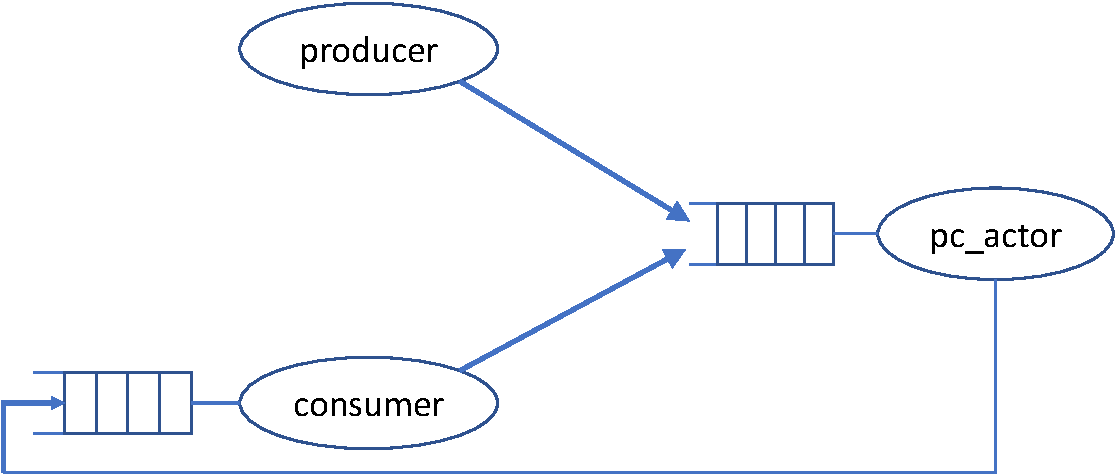
\includegraphics[width=4in]{figures/actor-crop.pdf}
\end{center}
\caption{Depiction of three actors.  The producer does not receive messages.}
\label{fig:actorpic}
\end{figure}

\begin{figure}
\begin{code}
\VerbatimInput[xleftmargin=5mm,numbers=left]{code/actor.cxl}
\end{code}
\caption{[actor.cxl] A producer/consumer actor.}
\label{fig:actor}
\end{figure}

\begin{figure}
\begin{code}
\VerbatimInput[xleftmargin=5mm,numbers=left]{code/actortest.cxl}
\end{code}
\caption{[actortest.cxl] Test code for producer/consumer actor.}
\label{fig:actortest}
\end{figure}

Some programming languages favor a different way of implementing
synchronization using so-called \emph{actors}~\cite{HBS73}.  Actors are
processes that have only private memory and communicate through message passing.
See Figure~\ref{fig:actorpic} for an illustration.
Given that there is no shared memory in the actor model (other than the message
queues, which have built-in synchronization), there is no need
for critical sections.  Instead, some sequential process owns a particular
piece of data and other processes access it by sending request messages
to the process and optionally waiting for response messages.  Each process
handles one message at a time, serializing all access to the data it owns.

The actor synchronization model is popular in a variety of programming
languages, including Erlang and Scala.  Actor support is also available
through popular libraries such as Akka, which is available for various
programming languages.  In Python, Java, and C/C++,
actors can be easily emulated using threads and \emph{synchronized queues}
\index{synchronized queue}
(aka \emph{blocking queues})
\index{blocking queue}
for messaging.
Each thread would have one such queue for receiving messages.
Dequeuing from an empty synchronized queue blocks the thread until
another thread enqueues a message on the queue.

The \texttt{synch} library supports a synchronized message queue,
similar to the \texttt{Queue} object in Python.
Its interface is as follows:
\begin{itemize}
\item \texttt{Queue()} returns a new message queue;
\item \texttt{enqueue(q, item)} adds \texttt{item} to the queue pointed to by \texttt{q};
\item \texttt{dequeue(q)} waits for and returns an item on the queue pointed to by \texttt{q}.
\end{itemize}

Note that a \texttt{Queue} behaves much like a zero-initialized semaphore.
\texttt{enqueue} is much like \texttt{V}, except that it is accompanied by data.
\texttt{dequeue} is much like \texttt{P}, except that it also returns data.
Thus, synchronized queues can be considered a generalization of counting semaphores.

Figure~\ref{fig:actor} shows a CXL solution to the producer/consumer problem
(with an unbounded buffer)
using an actor (as illustrated in Figure~\ref{fig:actorpic}.
\texttt{pc\_actor} is essentially a matchmaker: it matches
\texttt{.produce} requests with \texttt{.consume} requests.
Sometimes it may have buffered \texttt{.consume} requests and is waiting for
\texttt{.produce} requests, and sometimes it is vice versa.
The variable \texttt{balance} specifies what the situation is: if it is positive
then it has buffered \texttt{.produce} requests;
if it is negative
then it has buffered \texttt{.consume} requests.
Note that both \texttt{balance} and \texttt{requests} are variables that are
local to the \texttt{pc\_actor} process.

Each request message is a dictionary with two fields.  One of the fields is
\texttt{.type}, which either is \texttt{.produce} or \texttt{.consume}.
In case of \texttt{.produce}, the second field is \texttt{.item} and holds
the data that is produced.
In case of \texttt{.consume}, the second field is \texttt{.queue} and holds
a pointer to the queue where the response message must be enqueued.
\texttt{.produce} messages do not get a response.

The \texttt{pc\_actor} process has two arguments.  \texttt{q} is a pointer
to the queue on which it receives messages.  \texttt{nrequests} is the total
number of requests that it will handle.  We need the latter because in CXL
all processes are required to terminate.  In a more realistic implementation,
the \texttt{pc\_actor} would be in an infinite loop awaiting requests.

The \texttt{produce} method takes two arguments: a pointer to the queue
of the \texttt{pc\_actor} and the item.  The \texttt{consume} method
takes two queue pointer arguments.  The first is a pointer to the queue
of the \texttt{pc\_actor}.  The second is a pointer to the queue of the
invoker: it is the queue to which the response must be posted.

Figure~\ref{fig:actortest} shows how this code may be used.  It spawns
\texttt{NITEMS} producer and consumer processes.  Note that in that
case the \texttt{pc\_actor} is expected to receive \texttt{2 * NITEMS}
requests.

\section*{Exercises}
\begin{problems}
\item Implement a version of parallel qsort (see Example~\ref{ex:qsort})
using the actor model.  Use an actor for each worker as well as a main
actor that waits for each worker actor to have finished.
\item Actors and message queues are good for building pipelines.
Develop a pipeline that computes Mersenne primes (primes that are one less
than a factor of two).  Write four actors:
\begin{enumerate}
\item an actor that generates a sequence of integers 1 through \texttt{N};
\item an actor that receives integers and forwards only those that are prime;
\item an actor that receives integers and forwards only those that are one
less than a factor of two;
\item an actor that receives integers but otherwise ignores them.
\end{enumerate}
Configure two versions of the pipeline, one that first checks if a number
is prime and then if it is one less than a factor of two, the other
in the opposite order.  Which do you think is better?
\end{problems}

\chapter{Non-Blocking Synchronization}
\label{ch:nonblocking}
\index{non-blocking synchronization}
\glsadd{non-blocking synchronization}

\begin{figure}
\begin{code}
\VerbatimInput[xleftmargin=5mm,numbers=left]{code/hw.cxl}
\end{code}
\caption{[hw.cxl] Non-blocking queue.}
\label{fig:hw}
\end{figure}

So far we have concentrated on critical sections to synchronize multiple
processes.  Certainly, preventing multiple processes from accessing
certain code at the same time simplifies how to think about synchronization.
However, it can lead to starvation.  Even in the absence of starvation,
if some process is slow for some reason while being in the critical section,
the other processes have to wait for it to finish the critical section.
In this chapter, we will have a brief look at how one can develop concurrent
code in which processes never have to wait for other processes.
For this, we will revisit the producer/consumer problem, in which a
set of processes are producing items and a set of processes are
consuming items.

The code in Figure~\ref{fig:hw} is based on code developed by Herlihy and
Wing~\cite{HW87}.
The code is a ``proof of existence'' for non-blocking synchronization; it
is not necessarily practical.
There are two variables.  \texttt{items} is an unbounded array with each
entry initialized to \texttt{()}.  \texttt{back} is an index into the
array and points to the next slot where a new value is inserted.
The code uses two interlock instructions:
\begin{itemize}
\item \texttt{inc(p)}: atomically increments \texttt{\^{}p} and returns
the old value;
\item \texttt{swap(p)}: sets \texttt{\^{}p} to \texttt{()} and returns
the old value.
\end{itemize}

Method \texttt{produce(item)} uses \texttt{inc \&(back)} to allocate
the next available slot in the \texttt{items} array.
It stores the item as a singleton tuple.
Method \texttt{consume()} repeatedly scans the array, up to the
\texttt{back} index, trying to find an item to return.
To check an entry, it uses \texttt{swap()}
to atomically remove an item from a slot if there is one.
This way, if two or more processes attempt to extract an item from
the same slot, at most one will succeed.

There is no critical section.  If one process is executing instructions
very slowly, this does not negatively impact the other processes, as it
would with solutions based on critical sections.
On the contrary, it helps them because it creates less contention.

The solution is not practical because the \texttt{items} array must be
unbounded if an unbounded number of items may be produced.  Each slot
in the array is only used once, which is inefficient.  Also, the \texttt{inc}
and \texttt{swap} interlock instructions are not universally available
on existing hardware.
However, in the literature there are many examples of practical
non-blocking (aka \emph{wait-free})
\index{wait-free synchronization}
synchronization algorithms~\cite{}.

\chapter{Barrier Synchronization}
\label{ch:barrier}
\index{barrier synchronization}
\glsadd{barrier synchronization}

\begin{figure}
\begin{center}
\includegraphics[width=\textwidth]{figures/barrier-crop.pdf}
\end{center}
\caption{High-level state diagram specification of barrier synchronization
with three processes and two rounds.  The three numbers specify how many
rounds each process has completed.}
\label{fig:barrierdiagram}
\end{figure}

\begin{figure}
\begin{code}
\VerbatimInput[xleftmargin=5mm,numbers=left]{code/barrier.cxl}
\end{code}
\caption{[barrier.cxl] Barrier synchronization with semaphores.}
\label{fig:barrier}
\end{figure}

Barrier synchronization is a problem that comes up in high-performance
parallel computing, used, among others, for scalable simulation.
Barrier synchronization is almost the opposite of critical sections:
the intention is to get a group of processes to run some code at the
same time.
More precisely, the processes run in rounds.  At the end of each round
there is a so-called \emph{barrier} where processes wait until all
processes have completed the round.
For example, in an iterative matrix algorithm, the matrix may be
cut up into fragments.  During a round, one process runs for each
fragment concurrently.  The next round is not allowed to start
until all processes have completed operations on their fragment.

Figure~\ref{fig:barrierdiagram} shows a high-level depiction with three
processes.  Initially all processes are in round~0.  Then each process
can start and finish the round.  However, none of the processes can
progress to the next round until all processes have finished the
current round.

Counting semaphores work well for implementing barrier synchronization.
Figure~\ref{fig:barrier} shows an example.  There is a 0-initialized
semaphore for each of the \texttt{N} processes.
Before process $i$ enters a round, it first sends a signal to every
other process and then waits until it receives a signal from
every other process.  Process $i$ sends a signal to process $j$
by incrementing \texttt{sema[$j$]} (using \texttt{V}),
while process $i$ waits for a signal be decrementing \texttt{sema[$i$]}
(using \texttt{P}).

The \texttt{round} array is kept to check the correctness of this
approach.  Each process increments its entry every time it enters
a round.  If the algorithm is correct, it can never be that two processes
are more than one round apart.

\section*{Exercises}
\begin{problems}
\item See if you can implement barrier synchronization for $N$ processes
with just three semaphores.  Busy waiting is not allowed.  How about just two?
\end{problems}

\chapter{Networking: Alternating Bit Protocol}
\label{ch:abp}
\index{alternating bit protocol}

\begin{figure}
\begin{code}
\VerbatimInput[xleftmargin=5mm,numbers=left]{code/abp.cxl}
\end{code}
\caption{[abp.cxl] Alternating Bit Protocol.}
\label{fig:abp}
\end{figure}

\begin{figure}
\begin{code}
\VerbatimInput[xleftmargin=5mm,numbers=left]{code/abptest.cxl}
\end{code}
\caption{[abptest.cxl] Test code for alternating bit protocol.}
\label{fig:abptest}
\end{figure}

\bibliographystyle{alpha}
\bibliography{paper}

\appendix

\chapter{List of Values}

Chapter~\ref{ch:cxlmachine} provides an introduction to CXL values.
Below is a complete list of CXL value types with examples:

\vspace{1em}
\begin{tabular}{|l|l|}
\hline
Boolean & \texttt{False}, \texttt{True} \\
\hline
integers & \texttt{..., -2, -1, 0, 1, 2, ...} \\
\hline
Atom & \texttt{.example}, \texttt{.test1} \\
\hline
Program Counter & (method names are program counter constants) \\
\hline
Dictionary & \texttt{dict\{ .account: 12345, .valid: False \} } \\
\hline
Set & \texttt{\{ 1, 2, 3 \}, \{ False, .id, 3 \} } \\
\hline
Address & \texttt{\&lock, \&flags[2]} \\
\hline
Context & (generated by \texttt{stop} expression) \\
\hline
\end{tabular}
\vspace{1em}

Tuples, lists, strings, and bags are all special cases of dictionaries.
Both tuples and lists map indexes (starting at 0) to CXL values.
Their format is either \texttt{(e, e, ..., e,)} or
\texttt{[e, e, ..., e,]}.
If the tuple or list has two or more elements, then the final comma
is optional.
A string must be enclosed by double quotes and is represented as
a tuple of its characters.  Characters are one-character atoms.
A bag or multiset is a dictionary that maps a value to how many
times it occurs in the bag.

All CXL values are ordered with respect to one another.  First they
are ordered by type according to the table above.
So, for example, \texttt{\texttt{True} < 0 < .xyz < \{ 0 \})}.
Within types, the following rules apply:

\begin{itemize}
\item \texttt{False < True};
\item integers are ordered in the natural way;
\item atoms are lexicographically ordered;
\item program counters are ordered by their integer values;
\item dictionaries are first converted into a list of ordered (key, value)
pairs.  Then two dictionaries are lexicographically ordered by this
representation;
\item a set is first converted into an ordered list, then lexicographically
ordered;
\item an address is a list of atoms.  Addresses are lexicographically
ordered accordingly;
\item contexts (Appendix~\ref{app:context}) are ordered by hash.
\end{itemize}

\chapter{List of Operators}

CXL currently supports the following operators:

\vspace{1em}
\begin{tabular}{|l|l|}
\hline
\texttt{e == e} & two CXL values of the same type \\
\hline
\texttt{e != e} & two CXL values of the same type \\
\hline
\texttt{e < e} & any two CXL values \\
\hline
\texttt{e <= e} & any two CXL values \\
\hline
\texttt{e > e} & any two CXL values \\
\hline
\texttt{e >= e} & any two CXL values \\
\hline
\texttt{e and e and ...} & two or more Booleans \\
\hline
\texttt{e or e or ...} & two or more Booleans \\
\hline
\texttt{not e} & a Boolean \\
\hline
\texttt{-e} & an integer \\
\hline
\texttt{e + e + ...} & two or more integers, sets, or lists \\
\hline
\texttt{e - e} & two integers or sets \\
\hline
\texttt{e * e * ...} & two or more integers or sets \\
\hline
\texttt{e / e} & two integers (integer division) \\
\hline
\texttt{e \% e} & two integers (division remainder) \\
\hline
\texttt{e~..~e} & two integers \\
\hline
\texttt{e in e} & first is any CXL value, second is set \\
\hline
\texttt{e not in e} & first is any CXL value, second is set \\
\hline
\texttt{e if e else e} & middle \texttt{e} must be a Boolean \\
\hline
\texttt{\^{}e} & an address \\
\hline
\texttt{choose e} & a set \\
\hline
\texttt{min e} & a set \\
\hline
\texttt{max e} & a set \\
\hline
\texttt{cardinality e} & a set \\
\hline
\texttt{keys e} & a dictionary \\
\hline
\texttt{len e} & a dictionary (includes tuple or list) \\
\hline
\texttt{bagsize e} & a bag \\
\hline
\texttt{atLabel e} & atom (corresponding to a label) \\
\hline
\texttt{nametag e} & \texttt{e} must be \texttt{()} \\
\hline
\texttt{processes e} & \texttt{e} must be \texttt{()} \\
\hline
\texttt{\&lv} & \texttt{lv} is an lvalue \\
\hline
\texttt{stop lv} & \texttt{lv} is an lvalue \\
\hline
\end{tabular}
\vspace{1em}

\texttt{+} computes the union when applied to sets and
the concatenation when applied to lists or tuples.
\texttt{-} computes set difference when applied to two sets.
\texttt{*} computes the intersection when applied to sets.
\texttt{x..y} computes the set consisting of the integers \texttt{x}
through \texttt{y} inclusive.  It returns the empty set if \texttt{x > y}.

An \emph{lvalue}
\index{lvalue}
(short for left hand value of an assignment statement)
is something that can be assigned.  This can be a
shared variable, a process variable, or a dereferenced pointer
variable.  It can also be indexed.  Examples include
\texttt{var}, \texttt{var[e]}, and \texttt{\^{}p}.

CXL also supports the following comprehensions:

\vspace{1em}
\begin{tabular}{|l|l|}
\hline
Set comprehension & \texttt{\{ f(e) for e in s \}} \\
\hline
List comprehension & \texttt{[ f(e) for e in s ]} \\
\hline
Dict comprehension & \texttt{dict\{ f(e) for e in s \}} \\
\hline
\end{tabular}
\vspace{1em}

In each case, \texttt{s} must be a set.
For list comprehensions, the list will be sorted by \texttt{e}.
For dictionary comprehensions, each \texttt{e} will be mapped to \texttt{f(e)}.

\chapter{List of Statements}

CXL currently supports the following statements:

\vspace{1em}
\begin{tabular}{|l|l|}
\hline
\texttt{lv = e} & \texttt{lv} is an lvalue and \texttt{e} is an expression\\
\hline
\texttt{pass} & do nothing\\
\hline
\texttt{del lv} & delete\\
\hline
\texttt{assert b [, x]} & \texttt{b} is a Boolean.  If \texttt{False}, optionally print expression \texttt{e}\\
\hline
\texttt{const v = e} & \texttt{v} is an identifier, \texttt{e} is a constant expression\\
\hline
\texttt{def m(v, ...): S} & \texttt{m} and \texttt{v} are identifiers, \texttt{S} a list of statements\\
\hline
\texttt{let v = e, ...: S} & \texttt{e} is an expression, \texttt{S} a list of statements\\
\hline
\texttt{if b: S} & \texttt{b} is a Boolean, \texttt{S} a list of statements\\
\hline
\texttt{while b: S} & \texttt{b} is a Boolean, \texttt{S} a list of statements\\
\hline
\texttt{for v in e: S} & \texttt{e} is a set evaluated in order,
                            \texttt{S} a list of statements\\
\hline
\texttt{atomic: S} & \texttt{S} a list of statements\\
\hline
\texttt{spawn p e [, t]} & \texttt{p} is a method, \texttt{e} is an expression, \texttt{t} is an optional tag (an expression) \\
\hline
\texttt{go c e} & \texttt{c} is a context, \texttt{e} is an expression \\
\hline
\texttt{import m} & \texttt{m} identifies a module \\
\hline
\end{tabular}
\vspace{1em}

CXL does not support Python-style iterators.
To iterate through a dictionary, list, or tuple, use:
\texttt{for v in keys(e):~S}.

\chapter{List of Modules}
\label{ap:module}

The \texttt{bag} module
\index{bag module}
has various useful methods that operate on bags or
multisets:

\vspace{1em}
\begin{tabular}{|l|l|}
\hline
\texttt{bagEmpty()} & returns an empty bag\\
\hline
\texttt{bagFromset(s)} & create a bag from set \texttt{s}\\
\hline
\texttt{bagCount(b, e)} & count how many times \texttt{e} occurs in bag \texttt{b}\\
\hline
\texttt{bagChoose(b)} & like \texttt{choose(s)}, but applied to a bag\\
\hline
\texttt{bagAdd(pb, e)} & add one copy of \texttt{e} to bag \texttt{\^{}pb}\\
\hline
\texttt{bagRemove(pb, e)} & remove one copy of \texttt{e} from bag \texttt{\^{}pb}\\
\hline
\end{tabular}
\vspace{1em}

\noindent
\index{list module}
The \texttt{list} module has various useful methods that operate on lists
or tuples:

\vspace{1em}
\begin{tabular}{|l|l|}
\hline
\texttt{subseq(t, b, f)} & return a \emph{slice} of list \texttt{t} starting
at index \texttt{b} and ending just before index \texttt{f}\\
\hline
\texttt{append(t, e)} & append \texttt{e} to list \texttt{t}\\
\hline
\texttt{head(t)} & return the first element of list \texttt{t}\\
\hline
\texttt{tail(t)} & return all but the first element of list \texttt{t}\\
\hline
\texttt{qsort(t)} & sort list \texttt{t} using quicksort\\
\hline
\texttt{list2bag(t)} & convert list \texttt{t} into a bag \\
\hline
\texttt{list2set(t)} & convert list \texttt{t} into a set \\
\hline
\texttt{listMin(t)} & return the minimum of all elements in \texttt{t}\\
\hline
\texttt{listMax(t)} & return the maximum of all elements in \texttt{t}\\
\hline
\texttt{listSum(t)} & return the sum of all elements in \texttt{t}\\
\hline
\end{tabular}

\chapter{List of Machine Instructions}
\label{ap:cxlbytecode}

\vspace{1em}
\begin{tabular}{|l|l|}
\hline
Address & compute address \\
\hline
Apply & pop $m$ and $i$ and apply $i$ to $m$, pushing a value \\
\hline
Assert & pop $b$ and check that it is \texttt{True} \\
\hline
AtomicInc & increment the atomic counter of this context \\
\hline
AtomicDec & decrement the atomic counter of this context \\
\hline
Continue & no-op (but causes a context switch) \\
\hline
Choose & choose an element from the set on top of the stack \\
\hline
Del & delete a shared variable \\
\hline
DelVar $v$ & delete process variable $v$ \\
\hline
Dict & pop $n$ and $n$ key/value pairs and push a dictionary \\
\hline
Dup & duplicate the top element of the stack \\
\hline
Frame $m$($a$) end=$r$& start method $m$ with arguments $a$,
initializing variables.  Last instruction is at $r$ \\
\hline
Go & pop context and value, push value on context's stack, and add to context bag \\
\hline
Jump $p$ & set program counter to $p$ \\
\hline
JumpCond $e$ $p$ & pop expression and, if equal to $e$, set program counter to $p$ \\
\hline
Load $v$ & push shared variable $v$ (\texttt{\^} is indirect) onto the stack \\
\hline
LoadVar $v$ & load process variable $v$ and push it onto the stack \\
\hline
$n$-ary \textit{op} & apply $n$-ary operator \textit{op} to the top $n$ elements on the stack \\
\hline
Pop & pop a value of the stack and discard it \\
\hline
Push $c$ & push constant $c$ onto the stack \\
\hline
PushAddress $v$ & push the address of shared variable $v$ \\
\hline
Return & pop return address, push \texttt{result}, and restore program counter \\
\hline
Set & pop $n$ and $n$ elements and push a set of the elements \\
\hline
Spawn & pop tag, argument, and method and spawn a new context \\
\hline
Split & pop set and push minimum and remainder \\
\hline
Stop & save context into shared variable and remove from context bag \\
\hline
Store $v$ $[n]$ & pop a value from the stack and store it in shared variable $v$ (\texttt{\^} is indirect) \\
\hline
StoreVar $v$ & pop a value from the stack and store it in process variable $v$ \\
\hline
\end{tabular}
\vspace{1em}

Clarifications:
\begin{itemize}
\item The effect of the \texttt{Apply} instructions depends much on $m$.
If $m$ is a dictionary, then \texttt{Apply} finds $i$ in the dictionary
and pushes the value.
If $m$ is a program counter, then \texttt{Apply} invokes method $m$ by
pushing the current program counter and setting the program counter to
$m$.  $m$ is supposed to leave the result on the stack.
\item The \texttt{Frame} instruction pushes the value of the process
register (\emph{i.e.}, the values of the process variables) onto the
stack.  It initializes the \texttt{result} variable to the empty dictionary.
The \texttt{Return} instruction restores the process register by popping
its value of the stack.
\item All method calls have exactly one argument, although it sometimes
appears otherwise:
\begin{itemize}
\item \texttt{m()} invokes method \texttt{m} with the empty dictionary \texttt{()} as argument;
\item \texttt{m(a)} invokes method \texttt{m} with argument \texttt{a};
\item \texttt{m(a, b, c)} invokes method \texttt{m} with tuple \texttt{(a, b, c)} as argument.
\end{itemize}
The \texttt{Frame} instruction unpacks the argument to the method and places them into process variables by the given names.
\item Every \texttt{Stop} instruction must immediately be followed by a 
\texttt{Continue} instruction.
\end{itemize}

\chapter{Contexts and Processes}
\label{app:context}

A context captures the state of a process.  Each time the process
executes an instruction, it goes from one context to another.
All instructions update the program counter, and so no instruction
leaves the context the same.
There may be multiple processes
with the same state at the same time.

A context consists of the following:

\vspace{1em}
\begin{tabular}{|l|l|}
\hline
name tag & a dictionary with atoms \texttt{.name} and \texttt{.tag} \\
\hline
program counter & a Program Counter value pointing into the code \\
\hline
end & a Program Counter value indicating the end of the process code \\
\hline
atomic & if non-zero, the process is in atomic mode \\
\hline
stack & a list of CXL values \\
\hline
register & a CXL dictionary mapping atoms (representing process variables) to CXL values \\
\hline
stopped & a Boolean indicating if the context is stopped \\
\hline
\end{tabular}
\vspace{1em}

Details:
\begin{itemize}
\item The name in a name tag is the name of the method that the process
is executing;
\item The tag in a name tag is its argument by default.  Optionally
\texttt{spawn} allows the tag to be specified explicitly;
\item A process terminates when it reaches the \texttt{Return} instruction
of the method or when it hits a fault.  Faults include divide by zero,
reading a non-existent key in a dictionary, accessing a non-existent
variable, as well as when an assertion fails;
\item The execution of a process in atomic mode does not get interleaved
with that of other processes.
\item The register of a process always contains a dictionary, mapping
atoms to arbitrary values.  The atoms correspond to the variable names
in a CXL program.
\end{itemize}

A context is considered \emph{blocked}
\index{blocked process}
if there does not exist a
sequence instructions that the process can execute that either writes
to a shared variable (even if that leaves the shared variable unchanged)
or terminates the process.

\chapter{The CXL Virtual Machine}

The CXL Virtual Machine (CVM) has the following state:

\vspace{1em}
\begin{tabular}{|l|l|}
\hline
code & a list of CVM machine instructions \\
\hline
labels & a dictionary of atoms to program counters \\
\hline
variables & a dictionnary mapping atoms to values \\
\hline
ctxbag & a bag of non-stopped contexts \\
\hline
stopbag & a bag of stopped contexts \\
\hline
choosing & if not \texttt{None}, indicates a context that is choosing \\
\hline
failure & Boolean indicating some context has failed \\
\hline
initializing & Boolean indicating that the state is not fully initialized. \\
\hline
\end{tabular}
\vspace{1em}

There is initially a single context with nametag
\texttt{\_\_init\_\_/()} and program counter 0.  It starts executing
in atomic mode until it finishes executing the last instruction in
the code.  All states until then are \texttt{initializing} states.
Other processes, created through \texttt{spawn} statements, do not
start executing until then.

A \emph{micro step}
is the execution of a single CVM machine instruction
by a context.
Each micro step generates a new state.
When there are multiple contexts, the CVM can interleave them.
However, trying to interleave every microstep would be needlessly expensive,
as many micro steps involve changes to a context that are invisible to
other contexts.

A \emph{macro step}
\index{macro step}
can involve multiple micro steps.  The following
instructions start a new macro step: \texttt{Load}, \texttt{Store},
\texttt{AtomicInc}, and \texttt{Continue}.  The CVM
interleaves macro steps, not micro steps.  Like micro steps, each
macro step involves a single context.  Unlike a micro step, a macro
step can leave the state unchanged.

Executing a CXL program results in a graph where the nodes are CXL
states and the edges are macro steps.
When a state is \texttt{choosing}, the edges from that state are
by a single context, one for each choice.  If not, the edges from
the state are one per context.
A terminating state is a state with an empty context bag or a state
where all contexts are blocked.

\newpage
\printindex

\newpage
\printglossaries

\end{document}
